% !Mode:: "TeX:UTF-8" 
\renewcommand{\textfraction}{0.05} 
\BiChapter{实验要求}{}
本次实验的要求为对Lab1所完成的代码进行代码的评审以及性能分析,并从性能角度对代码进行优化。其中,代码的评审包括静态分析以及动态分析两个方面,并且在实验中逐一使用Checkstyle,FindBugs,PMD,VisualVM四个工具对代码进行评审以及性能分析。

在本次实验中,采用Lab1的分组方式(即两人一组),并随机分配另一组作为本组的评审和分析对象,并要求实验期间不能与原作者进行沟通。
% -------------------------------章节分割线-------------------------------
\BiChapter{在IntelliJ中配置代码审查与分析工具}{}
在本章中,将通过文字以及图片来对在IntelliJ中配置Checkstyle,PMD,FindBugs,VisualVM四种工具的步骤逐一进行叙述。
\BiSection{Checkstyle}{}
在本节中,将描述在IntelliJ中安装以及配置Checkstyle的方法。

首先,在IntelliJ中打开项目,然后在顶端的File选项栏中选择Setting选项,并在弹出的窗口中的左侧边栏中选择Plugins选项卡。
然后,在输入栏中输入“Checkstyle”,如图\ref{fig:cs-1}所示。

\begin{figure}
\centering
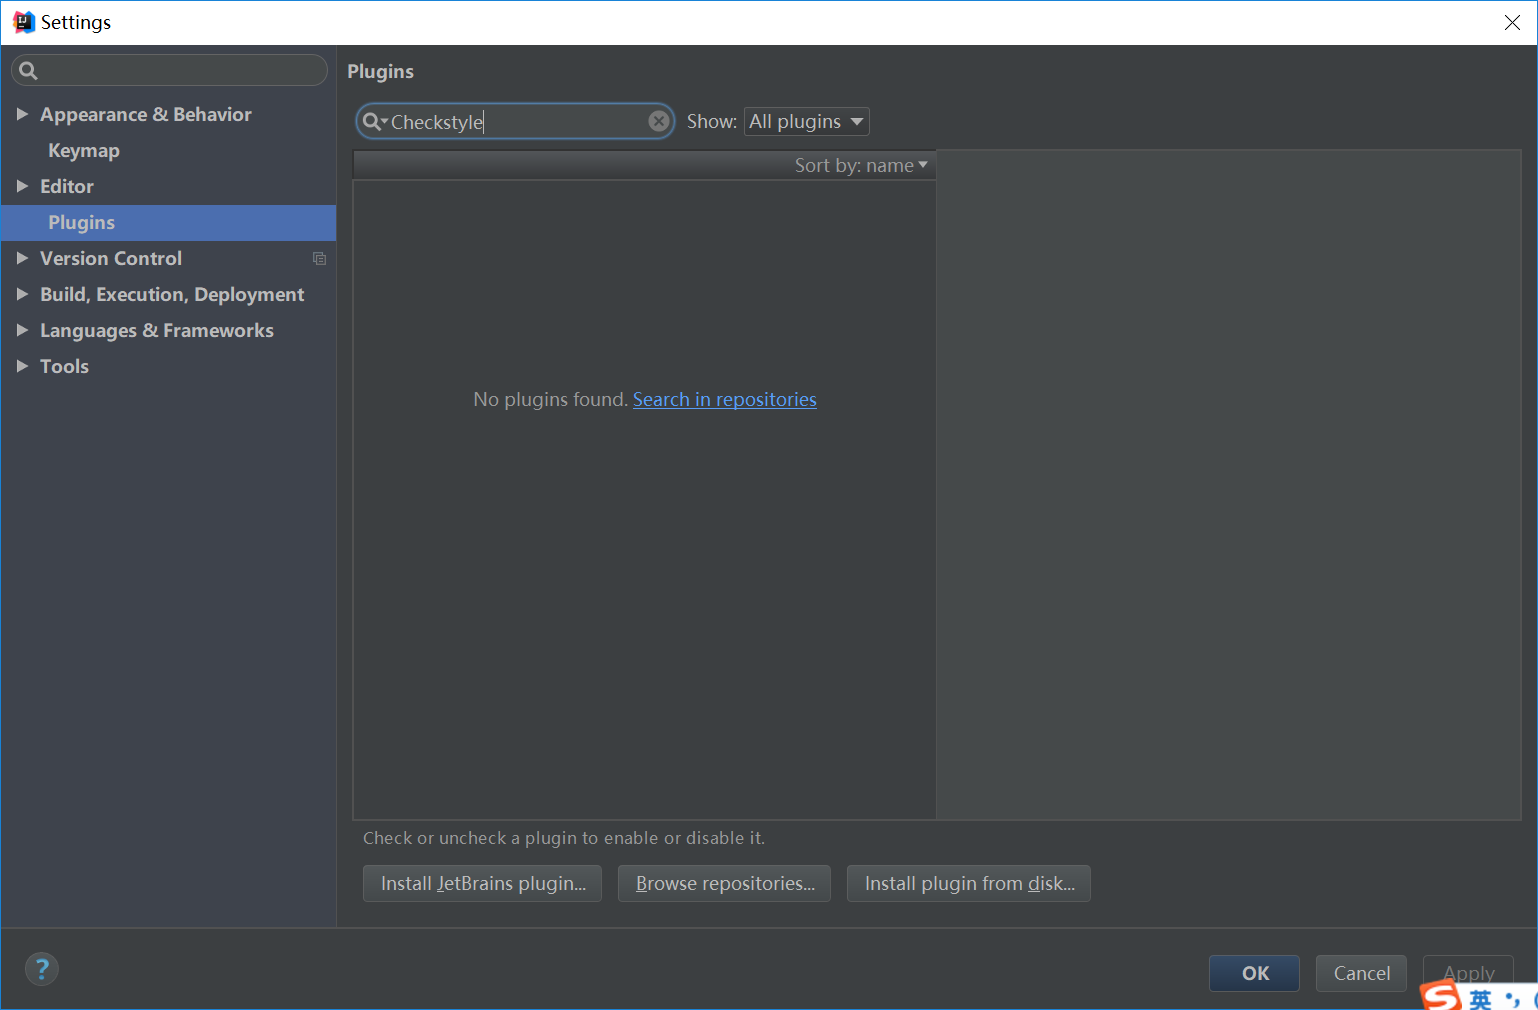
\includegraphics[width=12cm]{/../figures/cs-1}
\caption{Plugins选项卡}
\label{fig:cs-1}
\end{figure}

然后,点击其中的Search in repositories,在弹出的窗口中点击Install,如图\ref{fig:cs-2}所示。等待安装完成后,由此即完成了IntelliJ上Checkstyle的安装。

\begin{figure}
\centering
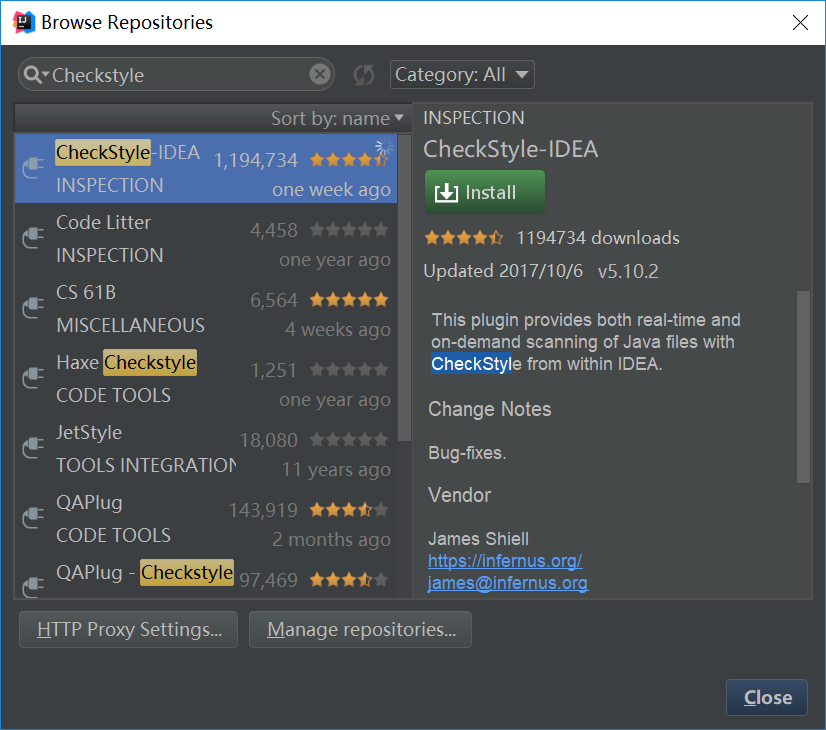
\includegraphics[width=10cm]{/../figures/cs-2}
\caption{Browse Repositories界面}
\label{fig:cs-2}
\end{figure}

在安装完成后,我们在Setting中左边栏选择Other Settings,Checkstyle。在出现的页面中的Configuration File选项中选择默认的Sun Checks作为风格检查的标准,如图\ref{fig:cs-3}所示,然后点击OK进行确定。由此,即完成了Checkstyle的配置。
\begin{figure}
\centering
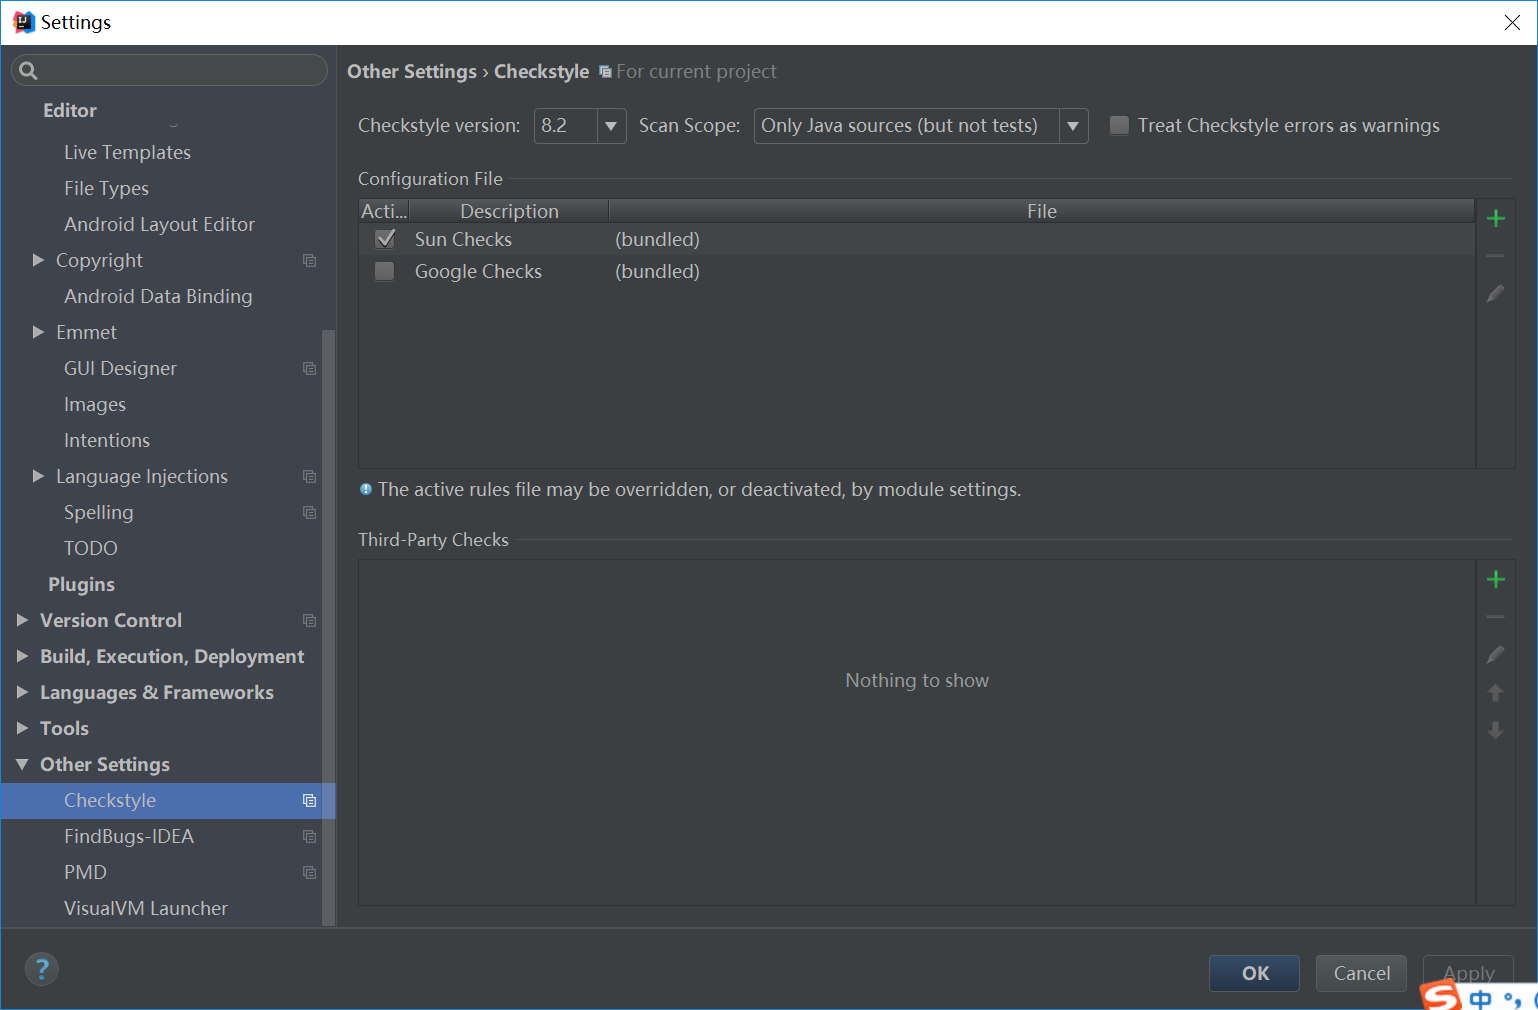
\includegraphics[width=12cm]{/../figures/cs-3}
\caption{设置检查标准}
\label{fig:cs-3}
\end{figure}

\BiSection{PMD}{}
在本节中,将描述在IntelliJ中安装以及配置PMD的方法。

与Checkstyle的安装方式基本一致,首先我们在Setting中的Plugins选项卡内输入“PMD”,点击Search in repositories,在出现的窗口中选择PMDPlugin,点击Install进行安装,等待安装完成。安装完后如图\ref{fig:pmd-1}所示。

\begin{figure}
\centering
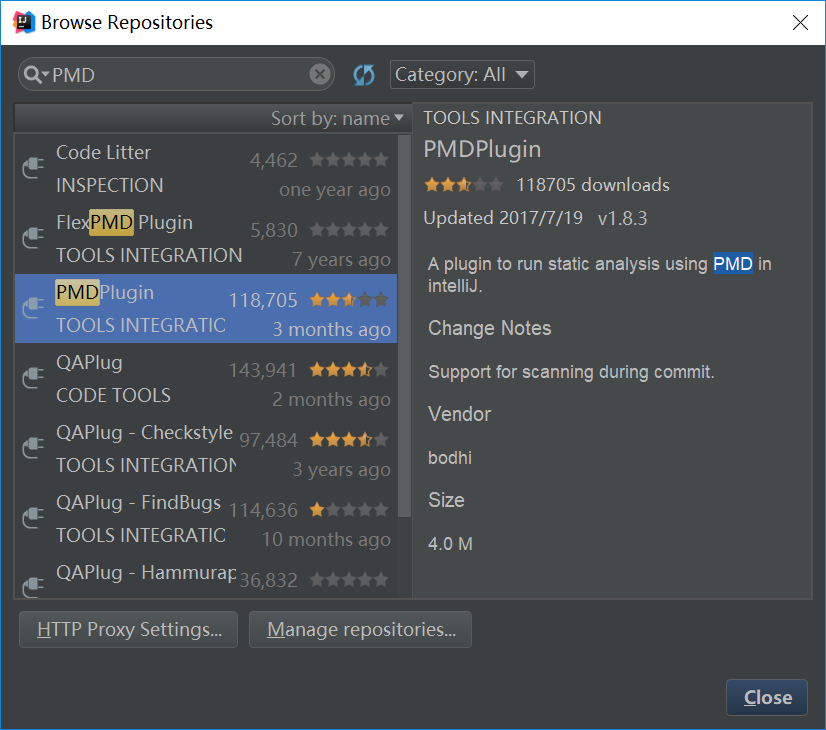
\includegraphics[width=10cm]{/../figures/pmd-1}
\caption{安装PMD}
\label{fig:pmd-1}
\end{figure}

由于本次实验中我们将直接使用PMD默认的配置,因此不需要进行额外的配置。

\BiSection{FindBugs}{}
在本节中,将描述在IntelliJ中安装FindBugs的方法。

与Checkstyle的安装方式基本一致,首先我们在Setting中的Plugins选项卡内输入“FindBugs”,点击Search in repositories,在出现的窗口中选择FindBugs-IDEA,点击Install进行安装,等待安装完成。安装完后如图\ref{fig:fb-1}所示。

\begin{figure}
\centering
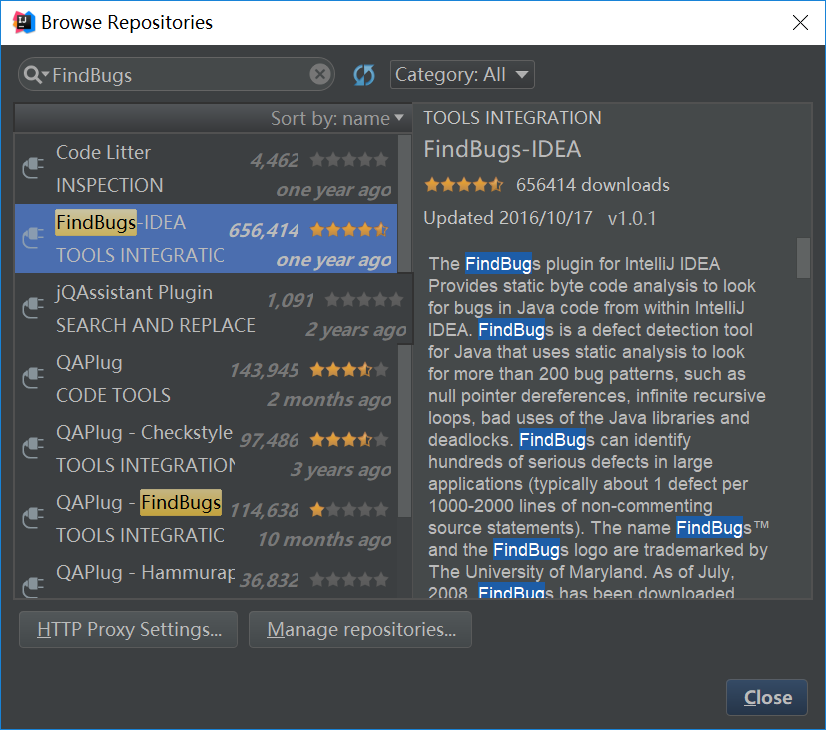
\includegraphics[width=10cm]{/../figures/fb-1}
\caption{安装FindBugs}
\label{fig:fb-1}
\end{figure}

\BiSection{VisualVM}{}
在本节中,将描述在IntelliJ中安装VisualVM的方法。

由于JDK中自带VisualVM软件,因此不需要额外安装VisualVM。不过,为了能够在IntelliJ中方便地使用VisualVM,我们选择安装VisualVM Launcher插件。该插件的安装过程与Checkstyle的安装方式基本一致,首先我们在Setting中的Plugins选项卡内输入“VisualVM”,点击Search in repositories,在出现的窗口中选择VisualVM Launcher,点击Install进行安装,等待安装完成。安装完后如图\ref{fig:vv-1}所示。

\begin{figure}
\centering
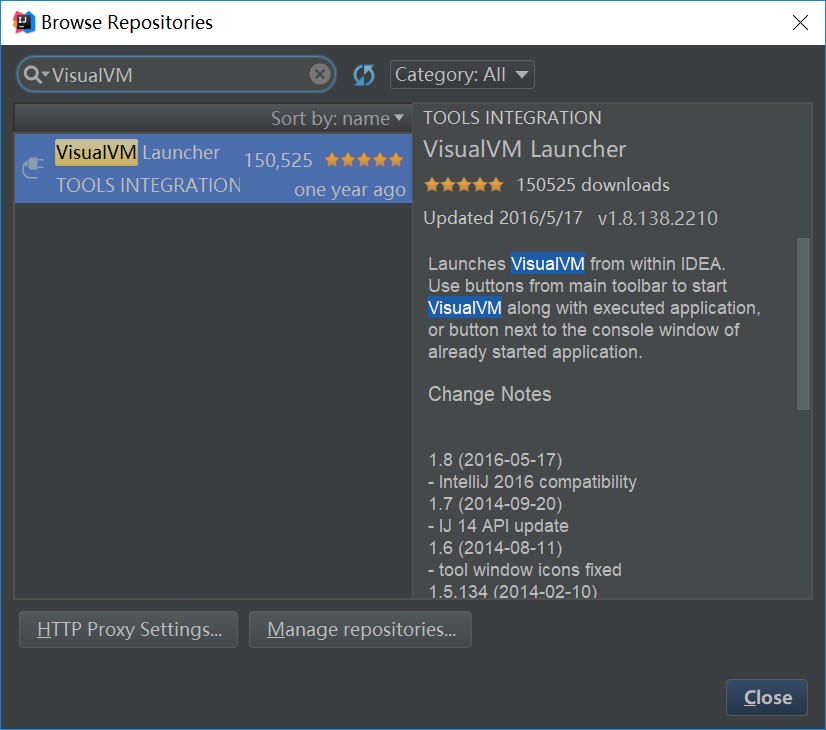
\includegraphics[width=10cm]{/../figures/vv-1}
\caption{VisualVM Launcher安装}
\label{fig:vv-1}
\end{figure}

% -------------------------------章节分割线-------------------------------
\BiChapter{本次实验所评审的代码}{}


\noindent 姓名:张冠华~\\
学号:1150310323~\\
Github地址:https://github.com/miuws~\\

\noindent 姓名:王珊~\\
学号:1150310302~\\
Github地址:https://github.com/arthua196
\begin{figure}[h]
\begin{center}
  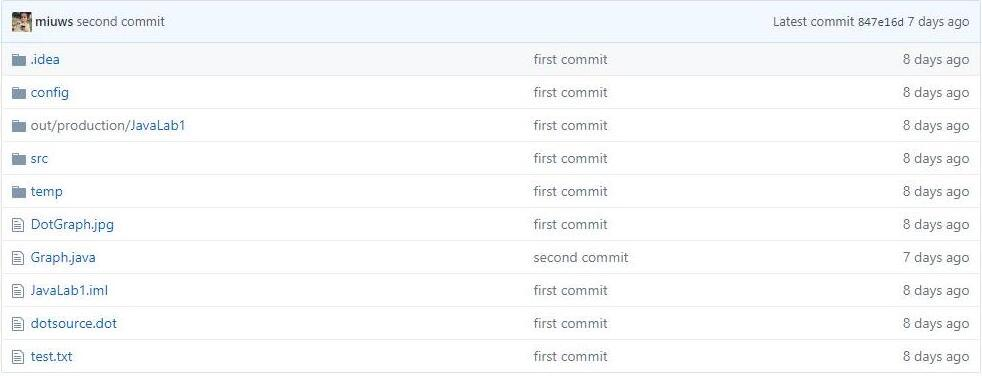
\includegraphics[width=\linewidth]{project.jpg}
  项目清单
\end{center}
\end{figure}

\begin{figure}[h]
\begin{center}
  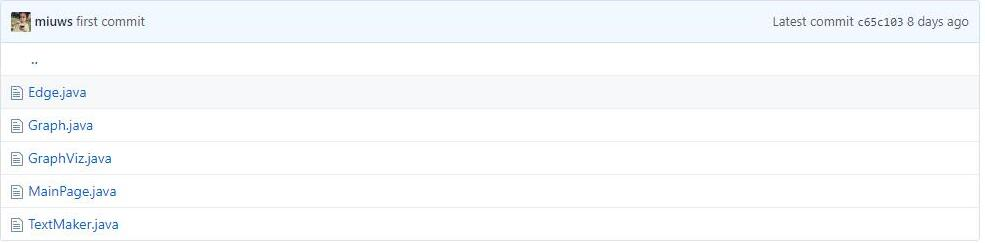
\includegraphics[width=\linewidth]{src.jpg}
  源码清单
\end{center}
\end{figure}


% -------------------------------章节分割线-------------------------------
\BiChapter{代码review记录}{}
\begin{adjustwidth}{-1pt}{}
\begin{tabular}{|c|c|c|c|}
\hline
 问题描述 & 类型 & 所在代码行号 &  修改方式\\
\hline
\makecell[l] {在点击退出按钮后 \\ GUI界面关闭 \\ 但程序仍在运行} & 
\makecell[l] {程序退出控制}  & 
\makecell[l] {MainPage.java \\ : 467} &
\makecell[l] {增加代码 \\ setDefaultCloseOperation \\ (WindowConstants. \\ EXIT\_ON\_CLOSE) }\\ 

\hline
\makecell[l] {没有对Graphviz \\ 关键字特别处理 \\ 展示图失败} & 
\makecell[l] {外部方法调用}  & 
\makecell[l] {TextMaker.java \\ : 168} &
\makecell[l] {使用引号 \\ 包围所有关键词 }\\ 

\hline
\makecell[l] {对文本逐字符处理 \\ 效率极低} & 
\makecell[l] {运行效率}  & 
\makecell[l] {TextMaker.java \\ : 53} &
\makecell[l] {使用一行正则表达式 \\ 完成文本处理} \\ 

\hline
\makecell[l] {重新打开对话框 \\ 以前输入的文字混乱} & 
\makecell[l] {GUI界面管理}  & 
\makecell[l] {MainPage.java \\ : 322} &
\makecell[l] {每次打开对话框 \\ 初始化新的对话框} \\ 


\hline
\makecell[l] {使用 \\ HIDE\_ON\_CLOSE \\ 关闭对话框} & 
\makecell[l] {GUI资源释放}  & 
\makecell[l] {MainPage.java \\ : 365} &
\makecell[l] {改为 \\ DISPOSE\_ON\_CLOSE} \\ 
\hline

\end{tabular}
\end{adjustwidth}


% -------------------------------章节分割线-------------------------------
\BiChapter{Checkstyle所发现的代码问题清单及原因分析}{}
\noindent
(使用 Sun Checks 规则)
~\\

\begin{adjustwidth}{-1pt}{}
\begin{tabular}{|c|c|c|c|c|}
\hline
编号 & 问题描述 & 类型 & 所在代码行号 & 修改策略 \\
\hline
1 &
\makecell[l] {类缺少JavaDoc} &
\makecell[l] {文档缺失} &
\makecell[l] {Edge.java \\ :3} &
\makecell[l] {补充Edge类文档} \\

\hline
2 &
\makecell[l] {大括号应位于 \\ 类、方法定义同一行} &
\makecell[l] {类、方法 \\ 定义格式} &
\makecell[l] {Edge.java \\ :4} &
\makecell[l] {将大括号放在 \\ 类、方法定义同一行} \\

\hline
3 &
\makecell[l] {','前缺少空格} &
\makecell[l] {空格格式} &
\makecell[l] {Edge.java \\ :5} &
\makecell[l] {补充空格} \\

\hline
4 &
\makecell[l] {应避免在 \\ 字表达式中赋值} &
\makecell[l] {赋值格式} &
\makecell[l] {Edge.java \\ :10} &
\makecell[l] {将赋值拆分成多行} \\

\hline
5 &
\makecell[l] {参数xxx应 \\ 定义为final的} &
\makecell[l] {只读参数、变量 \\ 用法} &
\makecell[l] {Edge.java \\ :12} &
\makecell[l] {为变量声明 \\ 增加final关键字} \\

\hline
6 &
\makecell[l] {'\{'后应换行} &
\makecell[l] {避免使用一行 \\ 定义方法} &
\makecell[l] {Edge.java \\ :33} &
\makecell[l] {为方法定义 \\ 规范换行} \\

\hline
7 &
\makecell[l] {if/else结构 \\ 必须使用大括号} &
\makecell[l] {控制结构 \\ 可读性} &
\makecell[l] {Edge.java \\ :36} &
\makecell[l] {为if结构 \\ 添加大括号} \\

\hline
8 &
\makecell[l] {数组大括号 \\ 位置错误} &
\makecell[l] {数组定义规范} &
\makecell[l] {Graph.java \\ :121} &
\makecell[l] {数组中括号 \\ 移至变量类型后} \\

\hline
9 &
\makecell[l] {xxx是一个 \\ 魔术数字} &
\makecell[l] {直接常数} &
\makecell[l] {Graph.java \\ :135} &
\makecell[l] {将数字赋值给常量} \\

\hline
10 &
\makecell[l] {不应以.*形式导入xxx} &
\makecell[l] {import规范} &
\makecell[l] {MainPage.java \\ :1} &
\makecell[l] {GUI使用了大部分 \\ 包中的类,不修改} \\

\hline
11 &
\makecell[l] {xxx应为private \\ 并配置访问方法} &
\makecell[l] {访问权限规范} &
\makecell[l] {MainPage.java \\ :13} &
\makecell[l] {访问权限改为private \\ 添加访问方法} \\

\hline
12 &
\makecell[l] {名称必须匹配 \\ 表达式xxx} &
\makecell[l] {命名规范} &
\makecell[l] {MainPage.java \\ :22} &
\makecell[l] {refactor修改命名} \\

\hline
13 &
\makecell[l] {本行字符数xxx \\ 最多xxx} &
\makecell[l] {行长度规范} &
\makecell[l] {MainPage.java \\ :80} &
\makecell[l] {拆成多行} \\
\hline

\end{tabular}
\end{adjustwidth}
~\\
(使用 Google 规则集的不同之处)
~\\
\begin{adjustwidth}{-1pt}{}
\begin{tabular}{|c|c|c|c|c|}
\hline
编号 & 问题描述 & 类型 & 所在代码行号 & 修改策略 \\
\hline
1 &
\makecell[l] {缩进空格应为两个} &
\makecell[l] {缩进格式} &
\makecell[l] {TextMaker.java \\ :13} &
\makecell[l] {(和规则集有关,不修改)} \\

\hline
2 &
\makecell[l] {包名导入顺序错误} &
\makecell[l] {import顺序错误} &
\makecell[l] {MainPage.java \\ :3} &
\makecell[l] {更改包导入顺序} \\

\hline
3 &
\makecell[l] {注释中的空行 \\  应该在<p>标签后} &
\makecell[l] {缩进格式} &
\makecell[l] {Graphviz.java \\ :23} &
\makecell[l] {(和规则集有关,不修改)} \\

\hline
4 &
\makecell[l] {其它if,for等 \\ 缩进空格数} &
\makecell[l] {缩进格式} &
\makecell[l] {Graph.java \\ :35} &
\makecell[l] {(和规则集有关,不修改)} \\
\hline
\end{tabular}
\end{adjustwidth}

~\\~\\
\noindent 小结:~\\
Sun和Google规则集大致相同。它们主要对这些问题进行检查:~\\
1、缩进~\\
2、有利于可读性的空格~\\
3、代码块是否正确地被大括号包围~\\

\noindent 不同的之处有:~\\
1、Google对缩进的要求是Sun规则集的一半~\\
2、Google规则集对JavaDoc的格式检查更严格~\\
3、Google规则集检查包名的导入顺序~\\
4、Sun规则集会检查部分内部逻辑


% -------------------------------章节分割线-------------------------------
\BiChapter{PMD所发现的代码问题清单及原因分析}{}
\noindent
优先级按照 https://pmd.github.io/pmd-5.8.1/pmd-java/rules/java 文档定义
~\\
\begin{adjustwidth}{-2em}{}
\begin{tabular}{|c|c|c|c|c|}
\hline
优先级 & 问题描述 & 违反的规则集合 & 代码行号 & 修改策略 \\
\hline
3 & 
\makecell[l] {变量、参数名过短 \\ 不易于理解} & 
\makecell[l] {naming} &
\makecell[l] {Edge.java \\ : 5} &
\makecell[l] {使用refactor \\ 更改命名} \\

\hline
3 & 
\makecell[l] {缺少包定义} & 
\makecell[l] {naming} &
\makecell[l] {Edge.java \\ : 3} &
\makecell[l] {为类编写文档} \\

\hline
4 & 
\makecell[l] {布尔型返回值 \\ 方法命名错误} & 
\makecell[l] {naming} &
\makecell[l] {Edge.java \\ : 33} &
\makecell[l] {用is、has、can等 \\ 命名此类方法} \\

\hline
3 & 
\makecell[l] {没有'\{'的if语句} & 
\makecell[l] {braces} &
\makecell[l] {Edge.java \\ : 46} &
\makecell[l] {为if结构增加'\{'} \\

\hline
3 & 
\makecell[l] {类中方法过多} & 
\makecell[l] {codesize} &
\makecell[l] {TextMaker.java \\ : 10} &
\makecell[l] {方法过多的类 \\ 应该重构} \\

\hline
3 & 
\makecell[l] {控制流程语句 \\ 过于复杂} & 
\makecell[l] {codesize} &
\makecell[l] {MainPage.java \\ : 69} &
\makecell[l] {重构以较少控制分支} \\

\hline
2 & 
\makecell[l] {缺少注释} & 
\makecell[l] {comments} &
\makecell[l] {Edge.java \\ : 3} &
\makecell[l] {添加注释} \\

\hline
3 & 
\makecell[l] {多个return的方法} & 
\makecell[l] {controversial} &
\makecell[l] {Edge.java \\ : 46} &
\makecell[l] {将返回值复制给变量 \\ 使用一个return返回} \\

\hline
3 & 
\makecell[l] {硬编码字面量} & 
\makecell[l] {controversial} &
\makecell[l] {Edge.java \\ : 46} &
\makecell[l] {赋予有意义的常量名} \\

\hline
3 & 
\makecell[l] {发现final局部变量} & 
\makecell[l] {controversial} &
\makecell[l] {Graph.java \\ : 51} &
\makecell[l] {将final局部变量 \\ 写成类的域} \\

\hline
3 & 
\makecell[l] {在操作数中赋值} & 
\makecell[l] {controversial} &
\makecell[l] {Graphviz.java \\ : 317} &
\makecell[l] {拆成多行,单独赋值} \\

\hline
3 & 
\makecell[l] {应显式指定访问权限} & 
\makecell[l] {controversial} &
\makecell[l] {MianPage.java \\ : 13} &
\makecell[l] {显示指定访问权限} \\

\hline
3 & 
\makecell[l] {使用具体实现的类 \\ 限制了功能的实现} & 
\makecell[l] {coupling} &
\makecell[l] {Graph.java \\ : 13} &
\makecell[l] {使用接口名 \\ 定义对象引用} \\
\hline
\end{tabular}
\end{adjustwidth}

~\\

\begin{adjustwidth}{-2em}{}
\begin{tabular}{|c|c|c|c|c|}
\hline
优先级 & 问题描述 & 违反的规则集合 & 代码行号 & 修改策略 \\
\hline
3 & 
\makecell[l] {只在初始化时赋值的 \\ 变量应声明为final} & 
\makecell[l] {design} &
\makecell[l] {Edge.java \\ : 4} &
\makecell[l] {在域中初始化 \\ 并声明为final} \\

\hline
3 & 
\makecell[l] {使用了size=0 \\ 判断集合是否为空} & 
\makecell[l] {design} &
\makecell[l] {Graph.java \\ : 155} &
\makecell[l] {使用isEmpty方法替代} \\

\hline
3 & 
\makecell[l] {发现God Class \\ (过于复杂的类)} & 
\makecell[l] {design} &
\makecell[l] {Graph.java \\ : 1} &
\makecell[l] {重构类} \\

\hline
3 & 
\makecell[l] {使用了'=' \\ 比较对象} & 
\makecell[l] {design} &
\makecell[l] {MainPage.java \\ : 74} &
\makecell[l] {替换为equals方法} \\

\hline
2 & 
\makecell[l] {发现空的catch代码块} & 
\makecell[l] {empty} &
\makecell[l] {TextMaker \\ : 136} &
\makecell[l] {抛出RuntimeException \\ 或处理异常} \\

\hline
3 & 
\makecell[l] {发现调用System.Exit} & 
\makecell[l] {j2ee} &
\makecell[l] {MainPage.java \\ : 216} &
\makecell[l] {检查逻辑 \\ System.Exit \\ 使用无误} \\

\hline
3 & 
\makecell[l] {发现可以声明 \\ 为final的参数} & 
\makecell[l] {optimizations} &
\makecell[l] {Edge.java \\ : 14} &
\makecell[l] {未在方法中修改的参数 \\ 声明为final} \\

\hline
3 & 
\makecell[l] {发现重复的字面量} & 
\makecell[l] {string} &
\makecell[l] {Graph.java \\ : 249} &
\makecell[l] {将字面量值赋予常量} \\

\hline
3 & 
\makecell[l] {发现未使用的参数} & 
\makecell[l] {unusedcode} &
\makecell[l] {Graph.java \\ : 85} &
\makecell[l] {删除参数} \\
\hline
\end{tabular}
\end{adjustwidth}

~\\
\noindent 小结:~\\
PMD的各个规则集都要它们自己的要检查的规则~\\
如naming规则集检查命名问题,design规则集检查代码的结构逻辑~\\
要根据规则集关于其规则的描述,决定是否应该使用规则集


% -------------------------------章节分割线-------------------------------
\BiChapter{FindBugs所发现的代码问清单及原因分析}{}

\begin{adjustwidth}{-1pt}{}
\begin{tabular}{|c|c|c|c|}
\hline
问题描述 & 类型 & 所在代码行号 & 修改策略 \\
\hline
\makecell[l] {不是所有的代码路径 \\ 都关闭了流} &
\makecell[l] {IO资源释放} &
\makecell[l] {Graphviz.java \\ : 315} &
\makecell[l] {try with resource \\ 管理资源} \\

\hline
\makecell[l] {try catch 语句 \\ catch未处理} &
\makecell[l] {异常处理} &
\makecell[l] {Graphviz.java \\ : 48} &
\makecell[l] {直接抛出异常或 \\ 在方法内处理异常} \\

\hline
\makecell[l] {使用$\backslash$ n作为换行符} &
\makecell[l] {格式化符号 \\ 符合平台特性} &
\makecell[l] {Graph.java \\ : 249} &
\makecell[l] {将$\backslash$ n替换为\%n} \\

\hline
\makecell[l] {发现调用 \\ System.exit} &
\makecell[l] {System.exit \\ 用法错误} &
\makecell[l] {Graph.java \\ : 216} &
\makecell[l] {检查逻辑 \\ System.Exit \\ 使用无误} \\

\hline
\makecell[l] {BufferedWriter  \\ 未指定编码} &
\makecell[l] {对默认编码依赖} &
\makecell[l] {Graphviz.java \\ : 254} &
\makecell[l] {针对平台 \\ 指定编码参数} \\

\hline
\makecell[l] {使用硬编码 \\ 引用绝对路径} &
\makecell[l] {使用硬编码} &
\makecell[l] {TextMaker.java \\ : 268} &
\makecell[l] {使用相对路径 \\ 并赋值给常量} \\
\hline

\end{tabular}
\end{adjustwidth}

% -------------------------------章节分割线-------------------------------
\BiChapter{VisualVM性能分析结果}{}
在本章中,将利用VisualVM工具对项目的执行时间以及内存占用情况进行分析,并根据分析得出的结果对项目代码进行改进。
最后将测试改进后的代码的执行时间以及内存占用情况,并与为改进之前的情况进行对比。

\BiSection{执行时间的统计结果与原因分析}{}
在本节中,将分别分析项目在生成与展示有向图,查询桥接词,根据桥接词生成新文本,计算两个单词之间的最短路径,以及随机游走这五个功能方面的耗时,并对耗时的原因进行分析。

需要说明的是,虽然在Lab1的原始要求中“读取并生成有向图”以及“展示有向图”为两个功能,但是在该项目中完成文件的读取以及有向图的生成后即自动展示了有向图,因此在此将原始要求中的两个功能需求合并为“读取并展示有向图”一个功能,并对这一个功能进行分析。

\BiSubsection{生成与展示有向图}{}
在生成与展示有向图的时间测试中,我们采用Lab1验收时的测试数据作为输入进行测试,耗时结果的统计见图\ref{fig:time-1}。

\begin{figure}
\centering
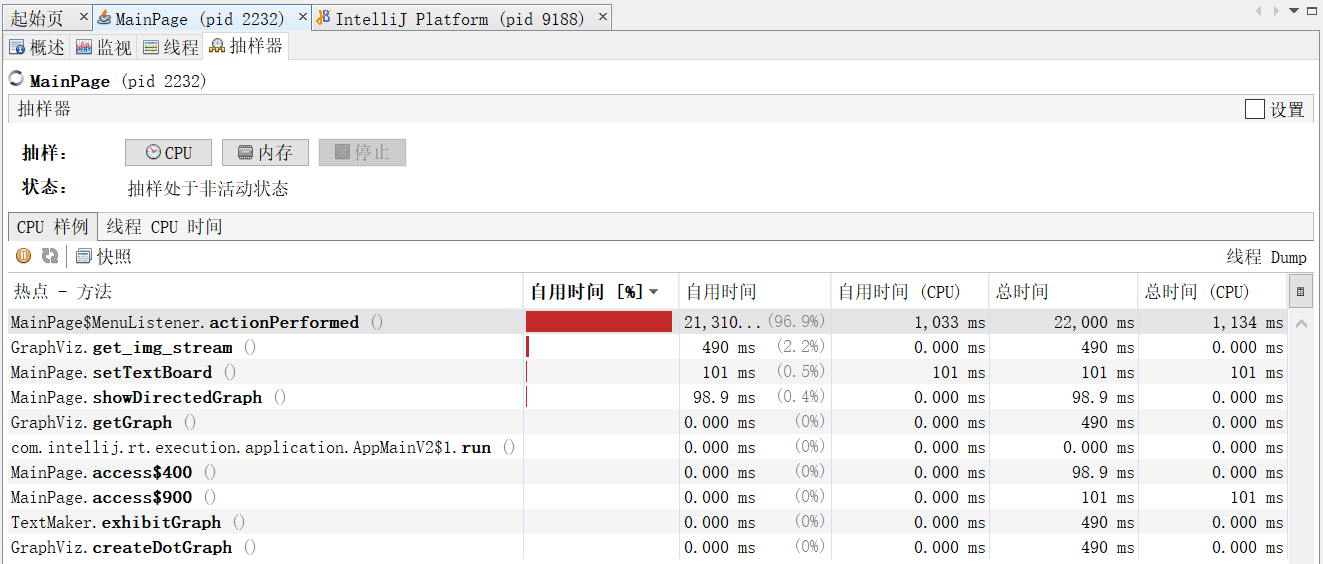
\includegraphics[width=12cm]{/../figures/time-1}
\caption{生成与展示有向图耗时}
\label{fig:time-1}
\end{figure}

需要首先特别说明的是,MenuListener.actionPerformed()的耗时为用户选择所要读取的文件时的耗时,因此不算在程序的运行时间内。

在耗时图像中,GraphViz.get\_img\_stream()为调用外部程序GraphViz绘制图像,并从GraphViz读取其返回的图像的二进制串的函数,GraphViz.createDotGraph()为接受GraphViz源程序作为输入,并最终将生成的图片写入到文件中的函数,TextMaker.exhibitGraph()为生成程序中图的结构对应的GraphViz源程序,并最终将生成的图片写入到文件中的函数,MainPage.setTextBoard()为配置GUI左侧展示文本框的函数,MainPage.showDirectedGraph()为配置GUI中展示有向图部分的GUI元素的函数。

由此可见,除去用户操作的时间外,主要占用时间的函数为GraphViz.get\_img\_stream(),MainPage.setTextBoard(),以及MainPage.showDirectedGraph()这三个函数。由于GraphViz.get\_img\_stream()为与GraphViz进行交互的函数,在不修改GraphViz的前提下没有更多优化的余地,并且MainPage.setTextBoard()与MainPage.showDirectedGraph()为控制GUI元素的函数,因此在使用同一GUI框架的前提下也无法进行优化,因此在生成与展示有向图的功能中无法通过耗时分析来进行这部分功能的优化。

\BiSubsection{查询桥接词}{}
在查询桥接词的测试中,我们同样采用Lab1验收的测试数据作为输入,即进行查询:
\begin{enumerate}
  \item 不存在的词的情况:first, second
  \item 不存在桥接词的情况:time, by
  \item 存在一个桥接词的情况:important, trends
  \item 存在多个桥接词的情况:the, of
\end{enumerate}
耗时分析结果见图\ref{fig:time-2}。

\begin{figure}
\centering
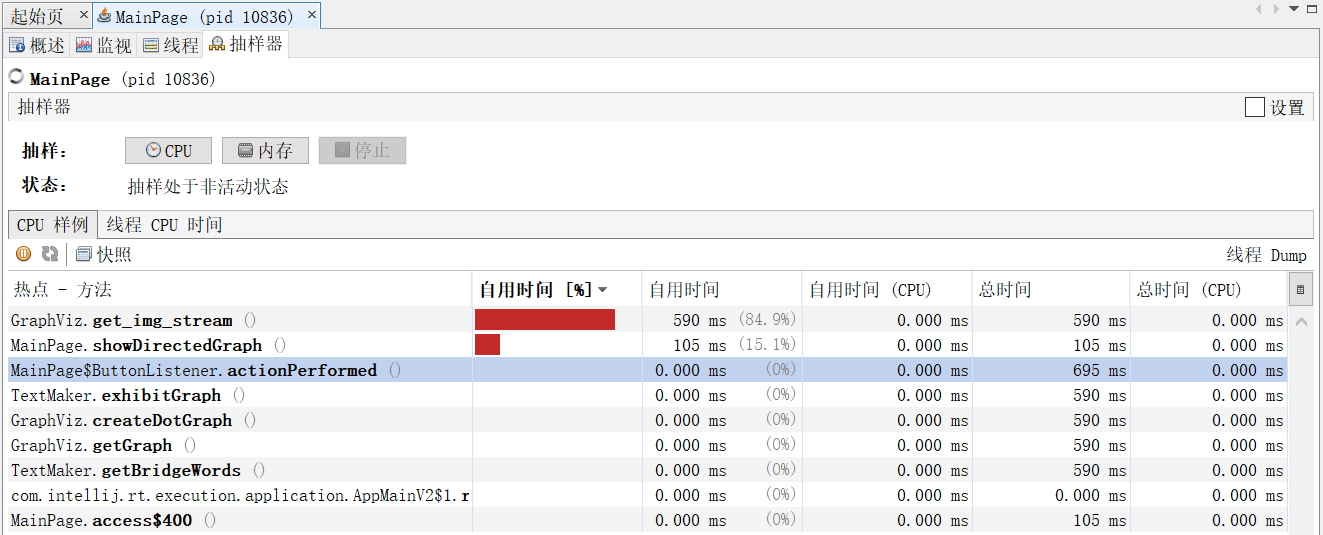
\includegraphics[width=12cm]{/../figures/time-2}
\caption{查询桥接词耗时分析}
\label{fig:time-2}
\end{figure}

在耗时图像中,GraphViz.get\_img\_stream()为调用外部程序GraphViz绘制图像,并从GraphViz读取其返回的图像的二进制串的函数,MainPage.showDirectedGraph()为配置GUI中展示有向图部分的GUI元素的函数,MainPage\$ButtonListener.actionPerformed()为处理按钮点击事件的函数,TextMaker.exhibitGraph()为生成程序中图的结构对应的GraphViz源程序,并最终将生成的图片写入到文件中的函数,GraphViz.createDotGraph()为接受GraphViz源程序作为输入,并最终将生成的图片写入到文件中的函数,GraphViz.getGraph()为接受GraphViz源程序作为输入,并将生成的图片的二进制返回的函数,TextMaker.getBridgeWords()为查询有向图中桥接词的函数。

由以上分析可见,在查询桥接词的过程之中,占用时间的主要是GraphViz.get\_img\_stream(),MainPage.showDirectedGraph()这两个函数。与生成并展示有向图时的情况相同,我们没法在不改变GUI框架以及GraphViz实现原理的情况下对这两个函数进行优化。

\BiSubsection{根据桥接词生成新文本}
在根据桥接词生成新文本的测试中,我们同样采用Lab1验收的测试数据作为输入,其输入的文本分别为“In the big time servitization becomes the of the world.”,以及“In the big time, servitization one of the important trends-of the IT world.”。测试得出的耗时图像见图\ref{fig:time-3}。

\begin{figure}
\centering
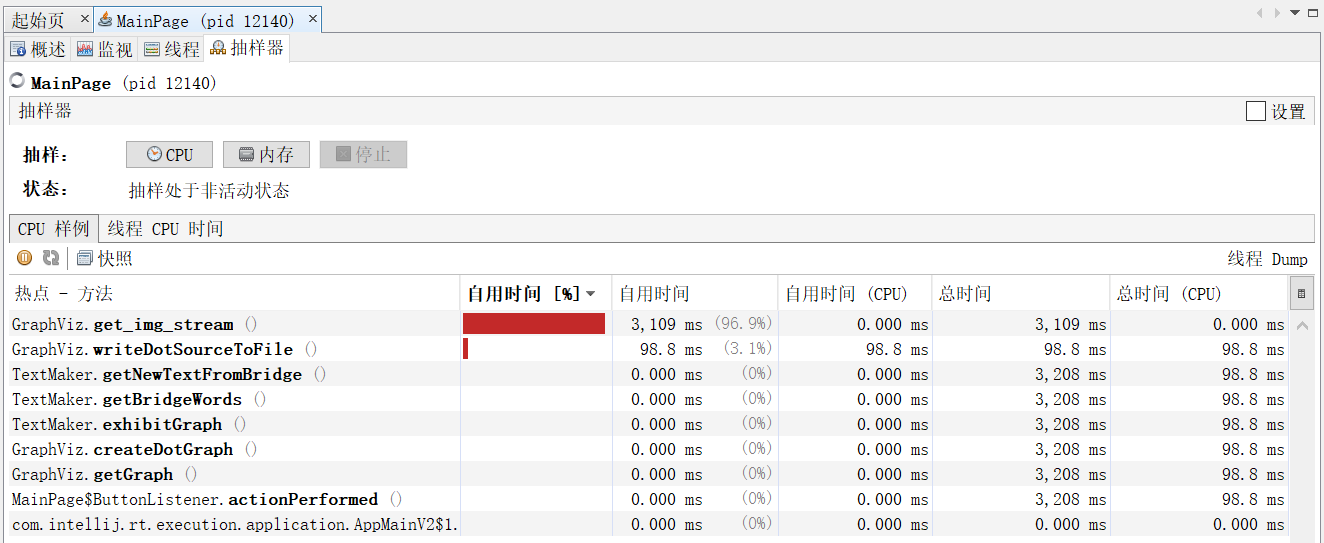
\includegraphics[width=12cm]{/../figures/time-3}
\caption{根据桥接词生成新文本耗时分析}
\label{fig:time-3}
\end{figure}

在耗时图像中,GraphViz.get\_img\_stream()为调用外部程序GraphViz绘制图像,并从GraphViz读取其返回的图像的二进制串的函数,GraphViz.writeDotSourceToFile()为接受GraphViz源代码作为输入,将源代码写入GraphViz源文件中的函数,MainPage\$ButtonListener.actionPerformed()为处理按钮点击事件的函数,TextMaker.exhibitGraph()为生成程序中图的结构对应的GraphViz源程序,并最终将生成的图片写入到文件中的函数,GraphViz.createDotGraph()为接受GraphViz源程序作为输入,并最终将生成的图片写入到文件中的函数,GraphViz.getGraph()为接受GraphViz源程序作为输入,并将生成的图片的二进制返回的函数,TextMaker.getBridgeWords()为查询有向图中桥接词的函数,TextMaker.getNewTextFromBridge()为根据输入的文本的桥接词生成新文本的函数。

由以上分析可知,占用时间的主要为GraphViz.get\_img\_stream(),GraphViz.writeDotSourceToFile()这两个函数。与之前分析的情况类似,在不改变通过GraphViz来生成图像的前提下,无法进一步从耗时方面提高程序的性能。

\BiSubsection{计算两个单词之间的最短路径}{}
在计算两个单词之间的最短路径的测试中,我们同样采用Lab1验收的测试数据作为输入,即测试:
\begin{enumerate}
\item 有一条最短路径的情况:time, word
\item 两个单词不可达的情况:this, study
\item 有多条最短路径的情况:the, word
\item 输入一个单词查询单源最短路径的情况:in
\end{enumerate}
测试得出的耗时图像见图\ref{fig:time-4}。

\begin{figure}
\centering
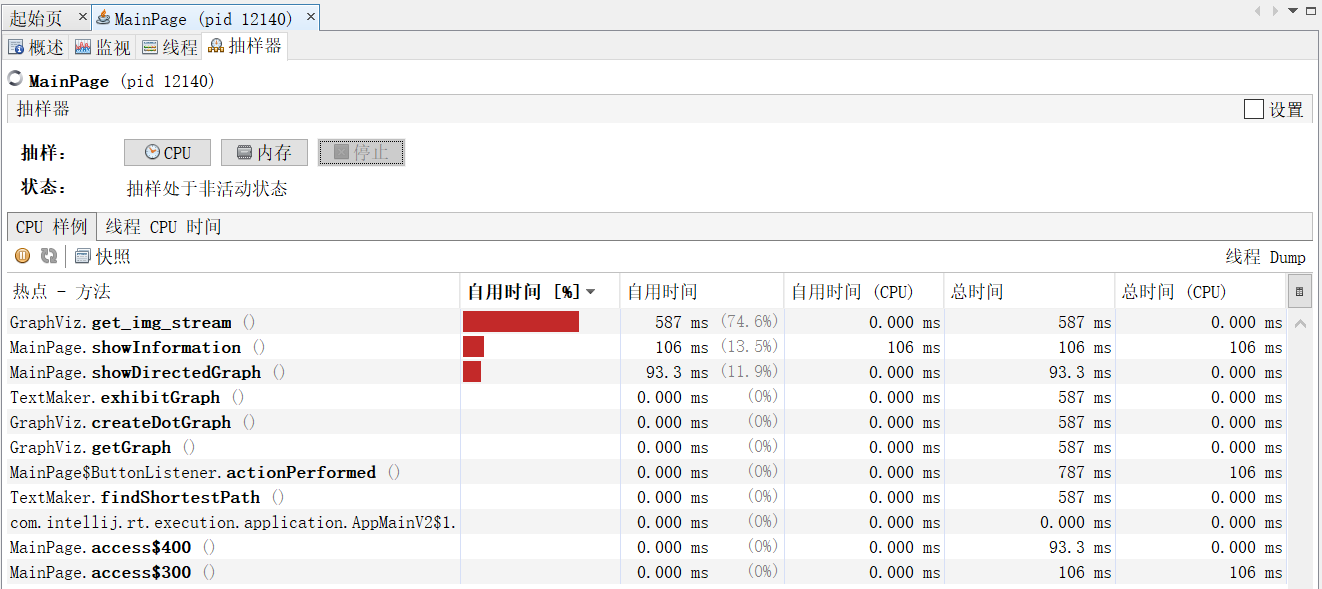
\includegraphics[width=12cm]{/../figures/time-4}
\caption{计算两个单词之间的最短路径耗时分析}
\label{fig:time-4}
\end{figure}

在耗时图像中,GraphViz.get\_img\_stream()为调用外部程序GraphViz绘制图像,并从GraphViz读取其返回的图像的二进制串的函数,MainPage.showInformation()为配置GUI中显示结果提示信息部分的GUI元素的函数,MainPage.showDirectedGraph()为配置GUI中展示有向图部分的GUI元素的函数,TextMaker.exhibitGraph()为生成程序中图的结构对应的GraphViz源程序,并最终将生成的图片写入到文件中的函数,GraphViz.createDotGraph()为接受GraphViz源程序作为输入,并最终将生成的图片写入到文件中的函数,GraphViz.getGraph()为接受GraphViz源程序作为输入,并将生成的图片的二进制返回的函数,MainPage\$ButtonListener.actionPerformed()为处理按钮点击事件的函数,TextMaker.findShortestPath()为查询单源最短路径的函数。

由以上分析可知,占用时间的主要是GraphViz.get\_img\_stream(),MainPage.showInformation(),MainPage.showDirectedGraph()这三个函数。与之前的情况相同,在不改变GUI框架以及使用GraphViz进行绘图的前提下无法从耗时方面对计算两个单词之间最短路劲的性能进行优化。

\BiSubsection{随机游走}{}
在随机游走的测试中不需要输入,其耗时图像见图\ref{fig:time-5}。

\begin{figure}
\centering
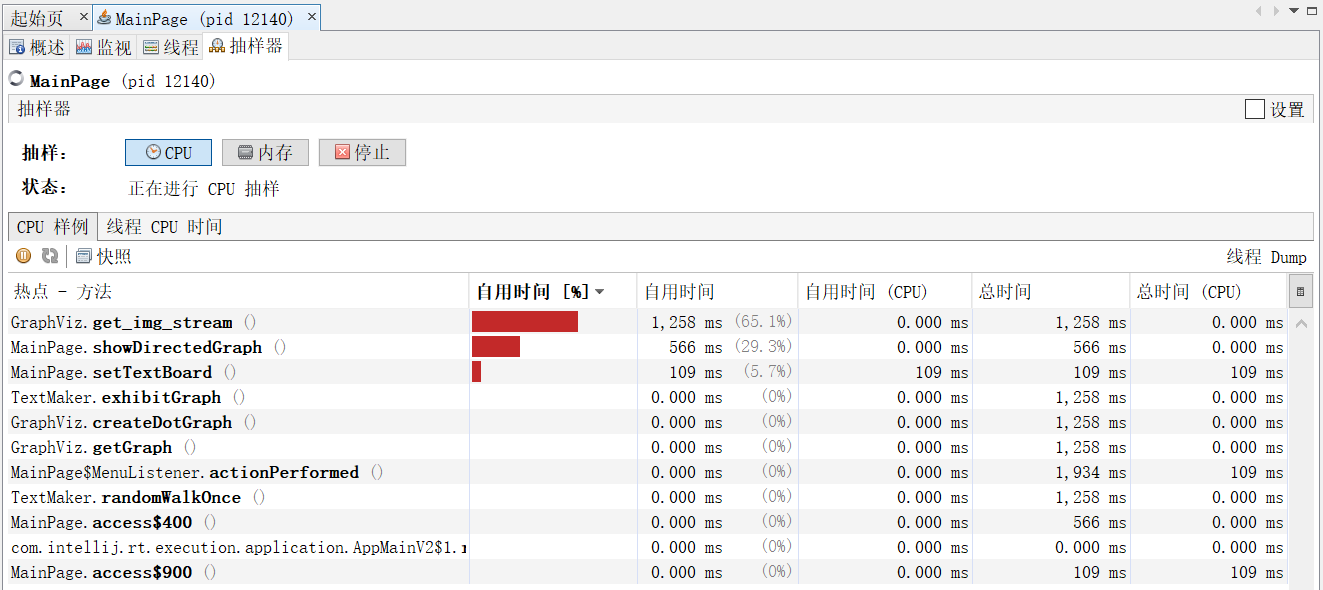
\includegraphics[width=12cm]{/../figures/time-5}
\caption{随机游走耗时分析}
\label{fig:time-5}
\end{figure}

在耗时图像中,GraphViz.get\_img\_stream()为调用外部程序GraphViz绘制图像,并从GraphViz读取其返回的图像的二进制串的函数,MainPage.showDirectedGraph()为配置GUI中展示有向图部分的GUI元素的函数,MainPage.setTextBoard()为配置GUI左侧展示文本框的函数,TextMaker.exhibitGraph()为生成程序中图的结构对应的GraphViz源程序,并最终将生成的图片写入到文件中的函数,GraphViz.createDotGraph()为接受GraphViz源程序作为输入,并最终将生成的图片写入到文件中的函数,GraphViz.getGraph()为接受GraphViz源程序作为输入,并将生成的图片的二进制返回的函数,MainPage\$ButtonListener.actionPerformed()为处理按钮点击事件的函数,TextMaker.findShortestPath()为查询单源最短路径的函数,TextMaker.randomWalkOnce()为随机游走一次的函数。

由以上分析可知,占用时间的主要是GraphViz.get\_img\_stream(),MainPage.showDirectedGraph(),MainPage.setTextBoard()三个函数。与之前的情况相同,在不改变GUI框架以及使用GraphViz进行绘图的前提下无法从耗时方面对计算两个单词之间最短路劲的性能进行优化。

\BiSection{内存占用的统计结果与原因分析}{}
在本节中,将分别分析项目在生成与展示有向图,查询桥接词,根据桥接词生成新文本,计算两个单词之间的最短路径,以及随机游走这五个功能方面的内存占用情况,并对占用内存的原因进行分析。

\BiSubsection{生成与展示有向图}{}
在生成与展示有向图部分,我们将主要考查多次读取输入文件时,是否发生了内存泄漏的情况。
测试的方法为分别记录读取一次文本,十次文本,二十次文本,三十次文本时的堆的使用情况,并进行比较。其中,每次读取使用相同的文本文件(也即Lab1的测试文件),并在每次记录数据前执行垃圾回收操作。由于程序每次读取文本时实际上在更新其内的有向图,并把原始文本以及预处理后的文本累加输出到GUI相应的文本框中,因此若无内存泄漏,则可预计java.lang.String在堆中的占用增加,其他类的占用应基本保持不变。

第一,二,三,四次记录的数据分别见图\ref{fig:mm-1-1},图\ref{fig:mm-1-2},图\ref{fig:mm-1-3},图\ref{fig:mm-1-4}。读取三十次文本时记录的数据与读取一次文本时记录的数据的差异比较见图\ref{fig:mm-1-5}。

\begin{figure}
\centering
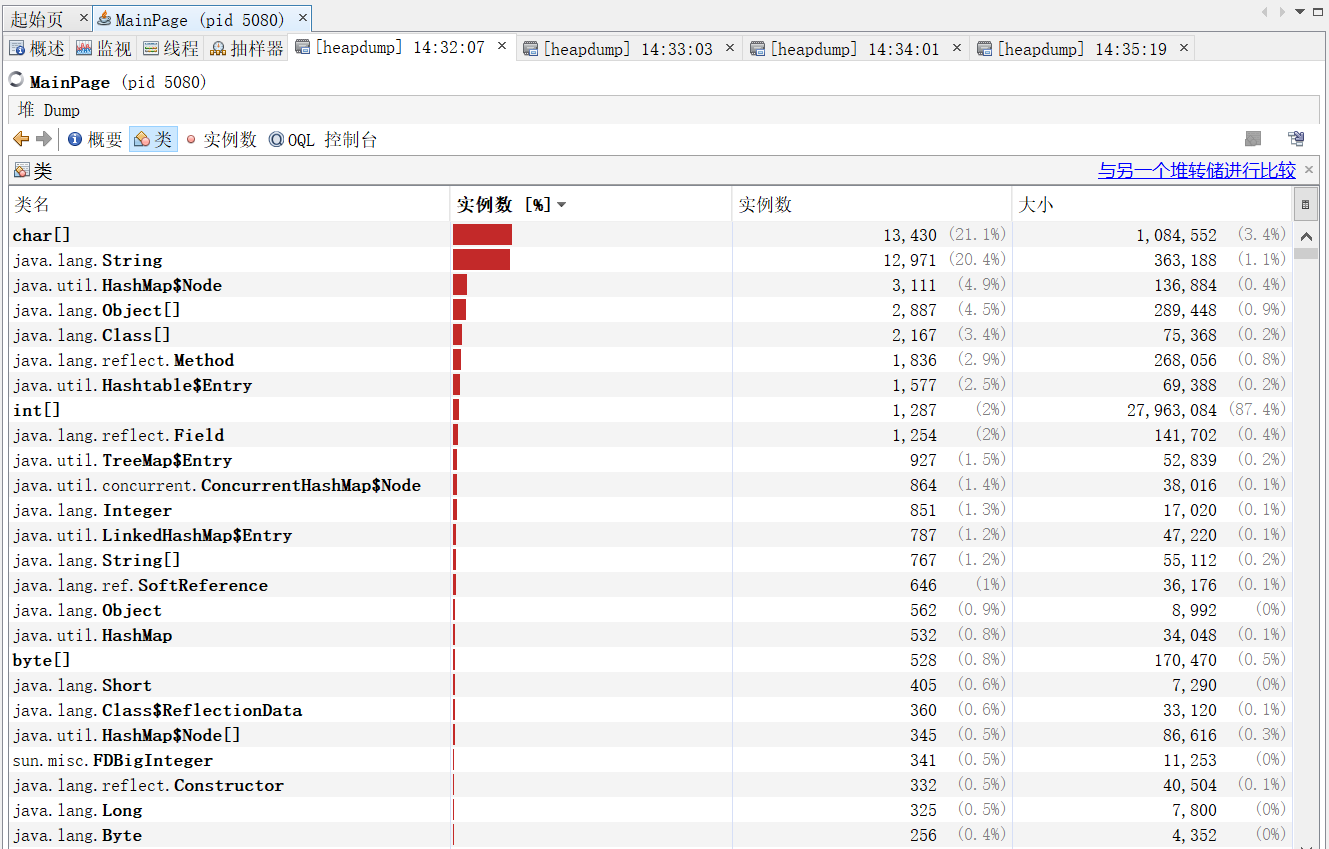
\includegraphics[width=12cm]{/../figures/mm-1-1}
\caption{读取一次文本时堆情况}
\label{fig:mm-1-1}
\end{figure}

\begin{figure}
\centering
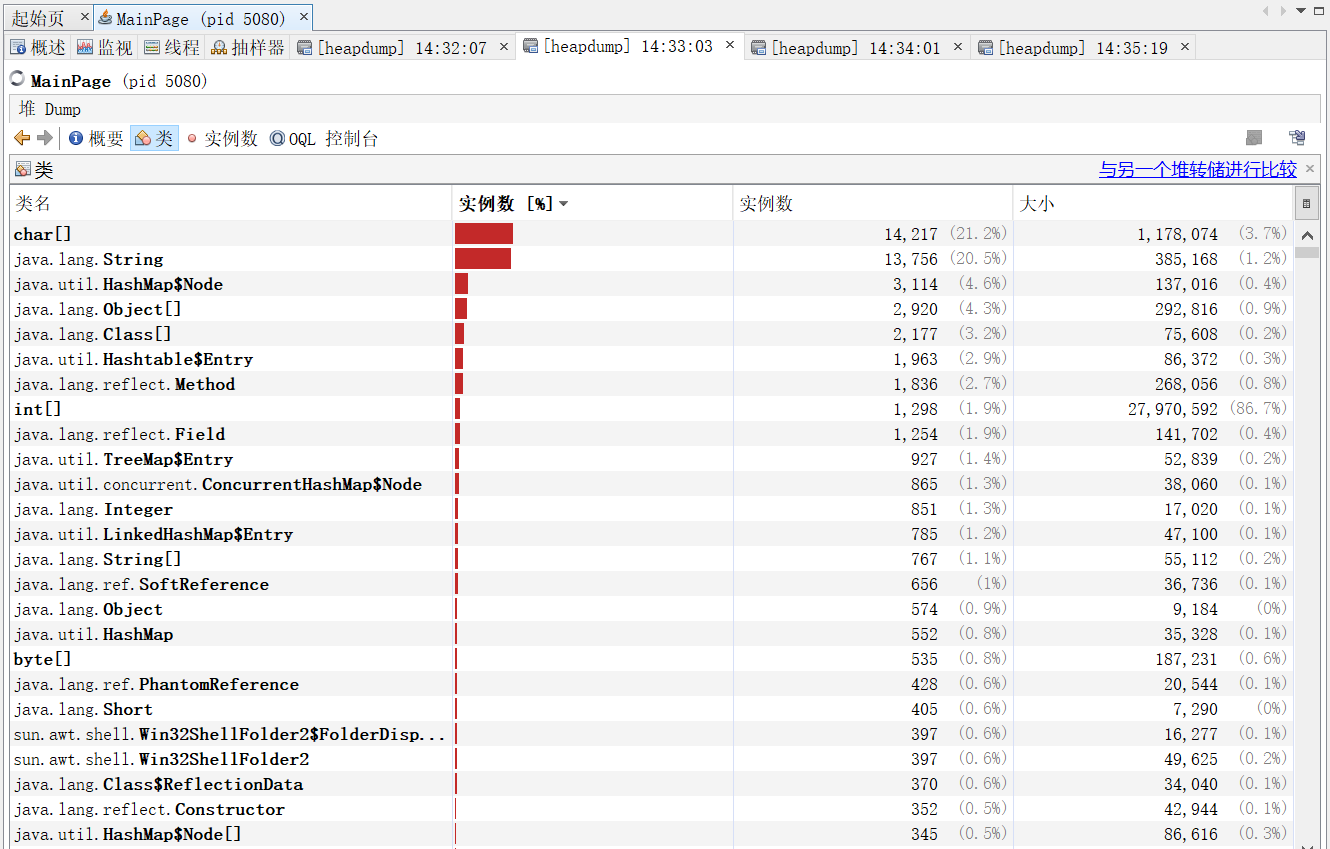
\includegraphics[width=12cm]{/../figures/mm-1-2}
\caption{读取十次文本时堆情况}
\label{fig:mm-1-2}
\end{figure}

\begin{figure}
\centering
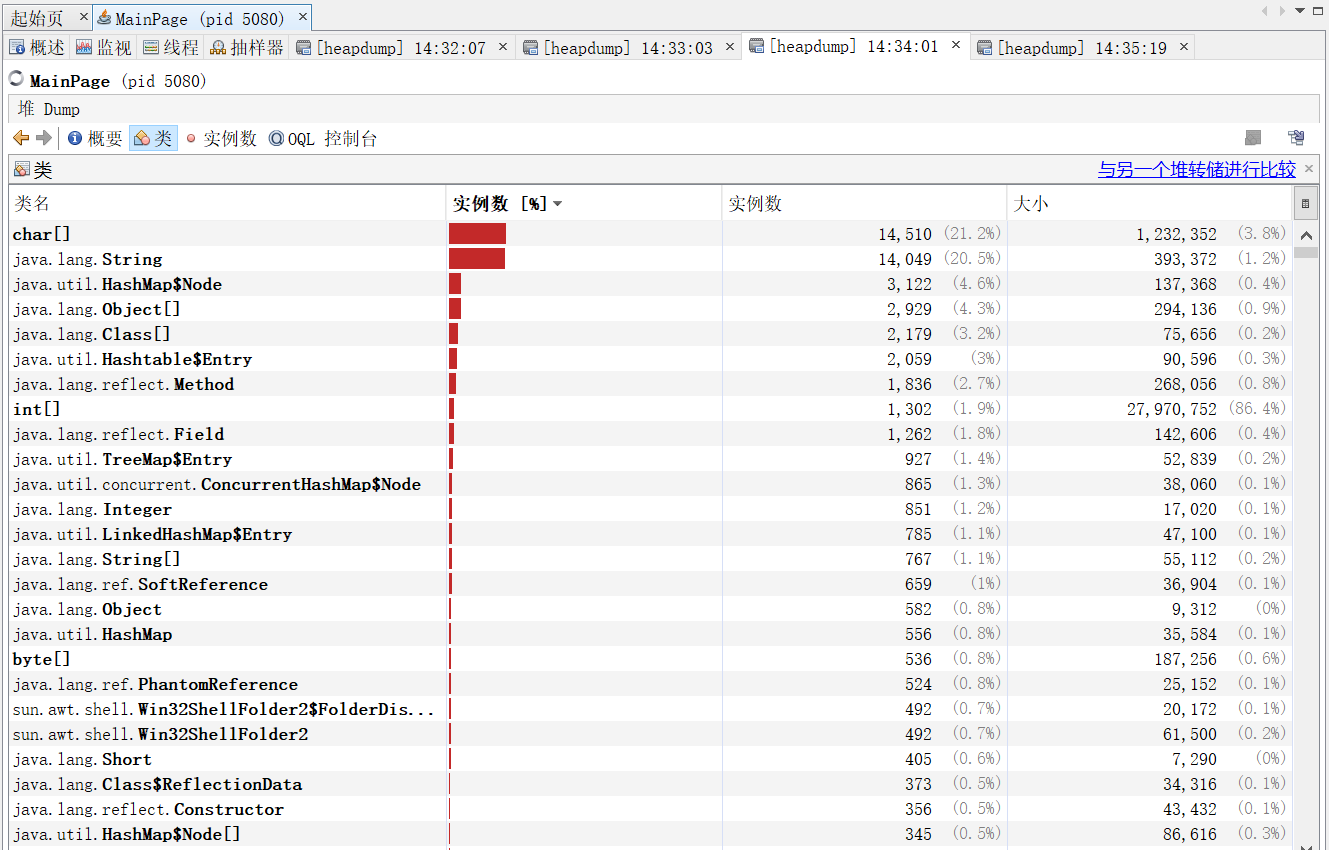
\includegraphics[width=12cm]{/../figures/mm-1-3}
\caption{读取二十次文本时堆情况}
\label{fig:mm-1-3}
\end{figure}

\begin{figure}
\centering
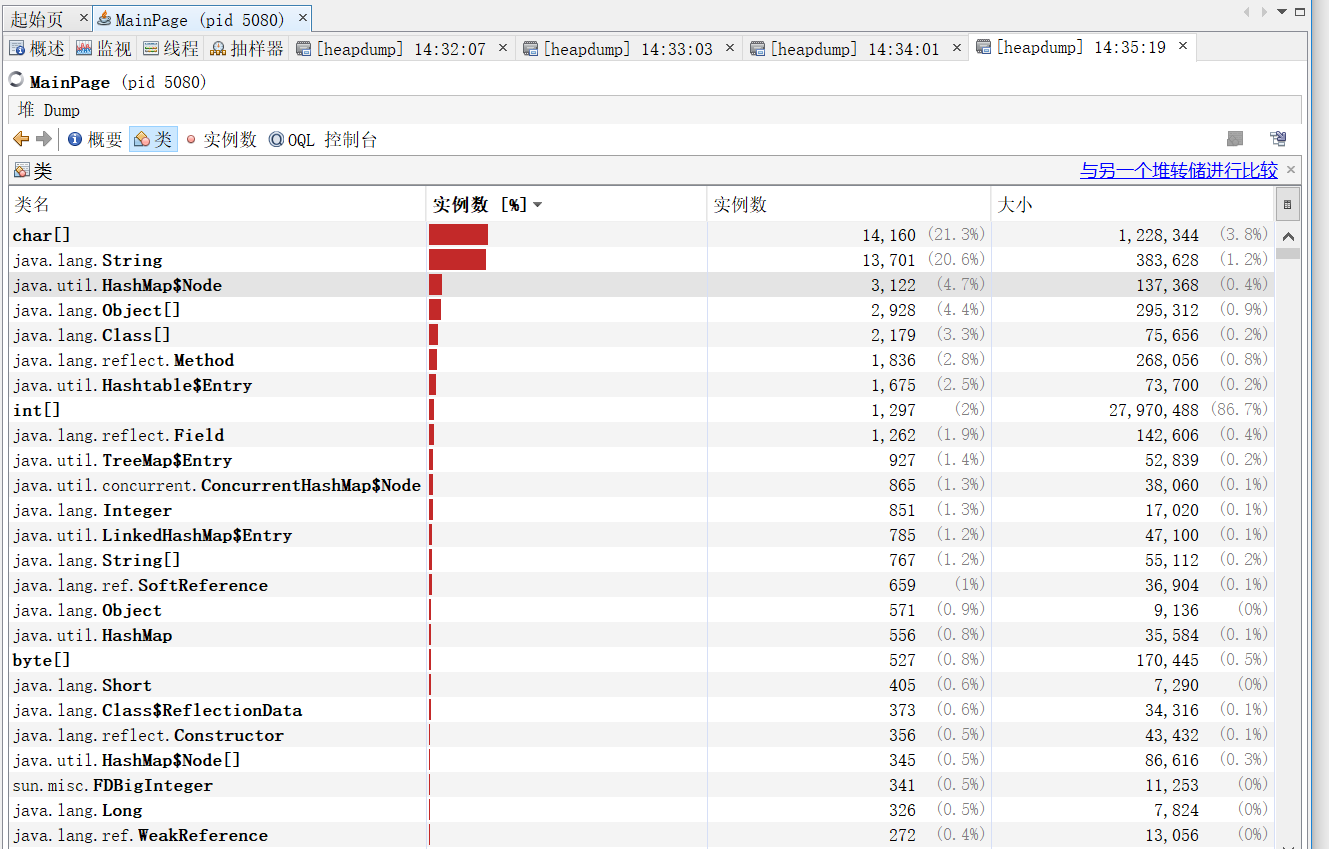
\includegraphics[width=12cm]{/../figures/mm-1-4}
\caption{读取三十次文本时堆情况}
\label{fig:mm-1-4}
\end{figure}

\begin{figure}
\centering
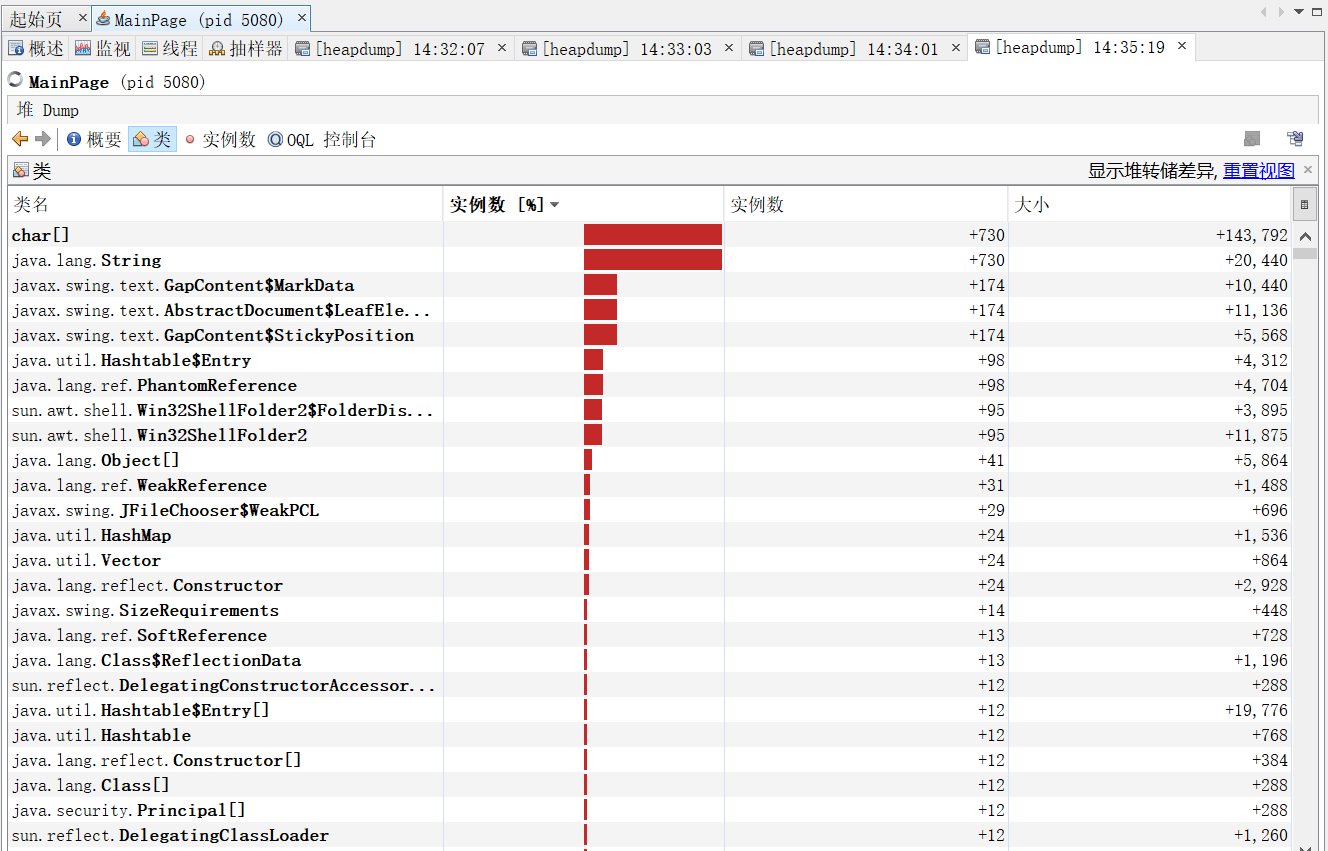
\includegraphics[width=12cm]{/../figures/mm-1-5}
\caption{读取三十次文本与读取一次文本比较}
\label{fig:mm-1-5}
\end{figure}

由图\ref{fig:mm-1-1},图\ref{fig:mm-1-2},图\ref{fig:mm-1-3},图\ref{fig:mm-1-4}可见,每次记录数据时主要占用堆空间的类为char[]以及java.lang.String,合起来每次记录数据时都占用了超过40\%的堆空间。另外,从图\ref{fig:mm-1-1}到图\ref{fig:mm-1-4}的变化中可以看出,每次记录数据时占用堆空间较多的类的实例数以及大小并没有发生较大的改变。由读取三十次文本与读取一次文本时堆的比较可见看出,char[]的实例数增加了5\%,java.lang.String的实例数增加了5\%,HashMap\$Node的实例数增加了0.3\%,即只有char[]以及java.lang.String两个类的占用发生了小幅度的提升,其他类的堆占用基本保持不变。这与无内存泄漏的预期结果相符合,因此可以推断此过程中未发生内存泄漏。

\BiSubsection{查询桥接词}{}
在查询桥接词的功能中,我们主要测试多次查询桥接词时是否会出现内存泄漏的情况。
测试方法为读入Lab1测试数据中“读取并生成有向图”部分的文件数据,然后在此有向图上进行一次,十次,二十次查询有多个桥接词的两个单词the,of之间的桥接词,由此分析是否在查询桥接词的过程中发生了内存泄漏。其中,每次记录堆的数据占用情况前都进行垃圾回收。
由于程序每次完成桥接词的查询之后通过弹出对话框的方式显示查询到的桥接词,关闭对话框后查询结果即消失,因此若无内存泄漏,则可预计所有类的堆占用情况皆不会发生较大的改变。

第一,二,三次记录的数据分别见图\ref{fig:mm-2-1},图\ref{fig:mm-2-2},图\ref{fig:mm-2-3}。查询二十次桥接词时记录的数据与查询一次桥接词时记录的数据的差异比较见图\ref{fig:mm-2-4}。

\begin{figure}
\centering
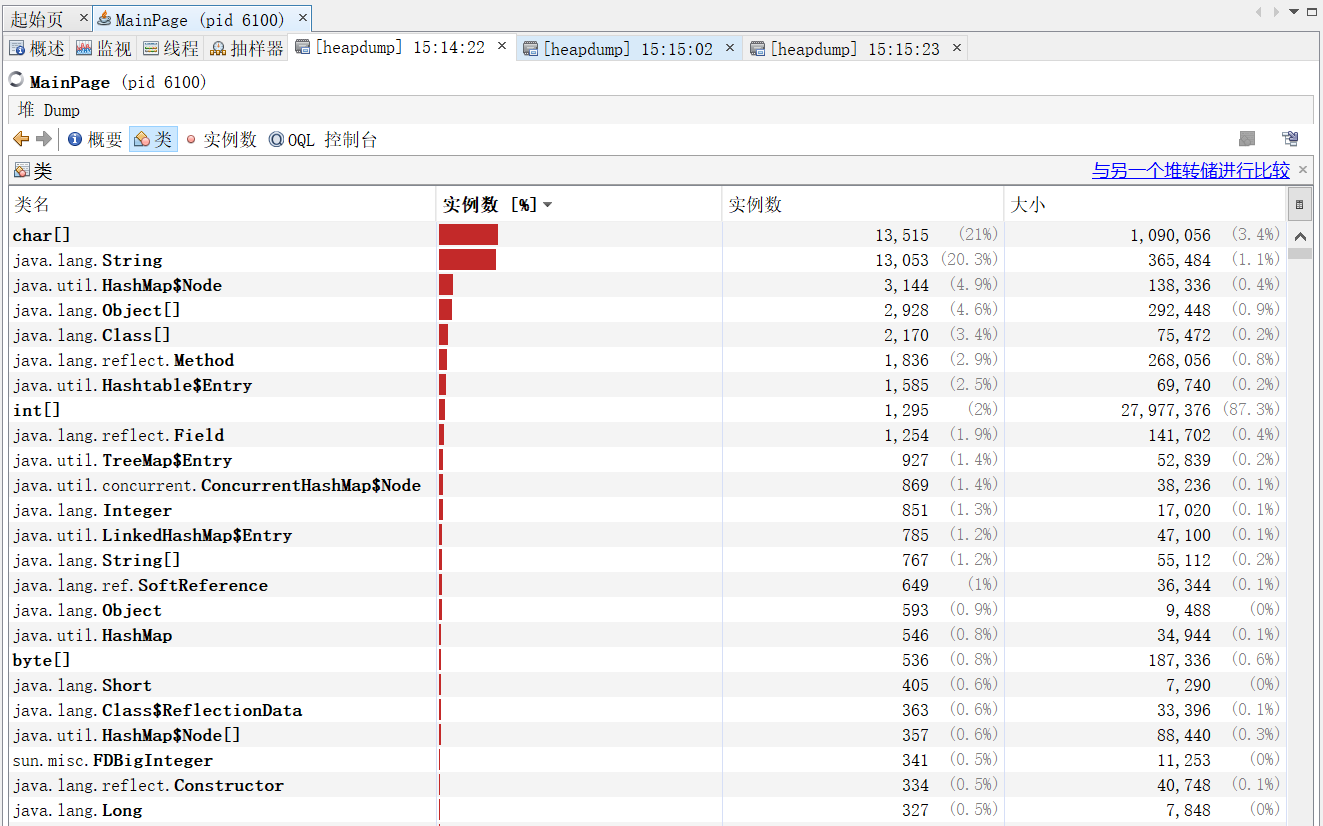
\includegraphics[width=12cm]{/../figures/mm-2-1}
\caption{查询一次桥接词时堆情况}
\label{fig:mm-2-1}
\end{figure}

\begin{figure}
\centering
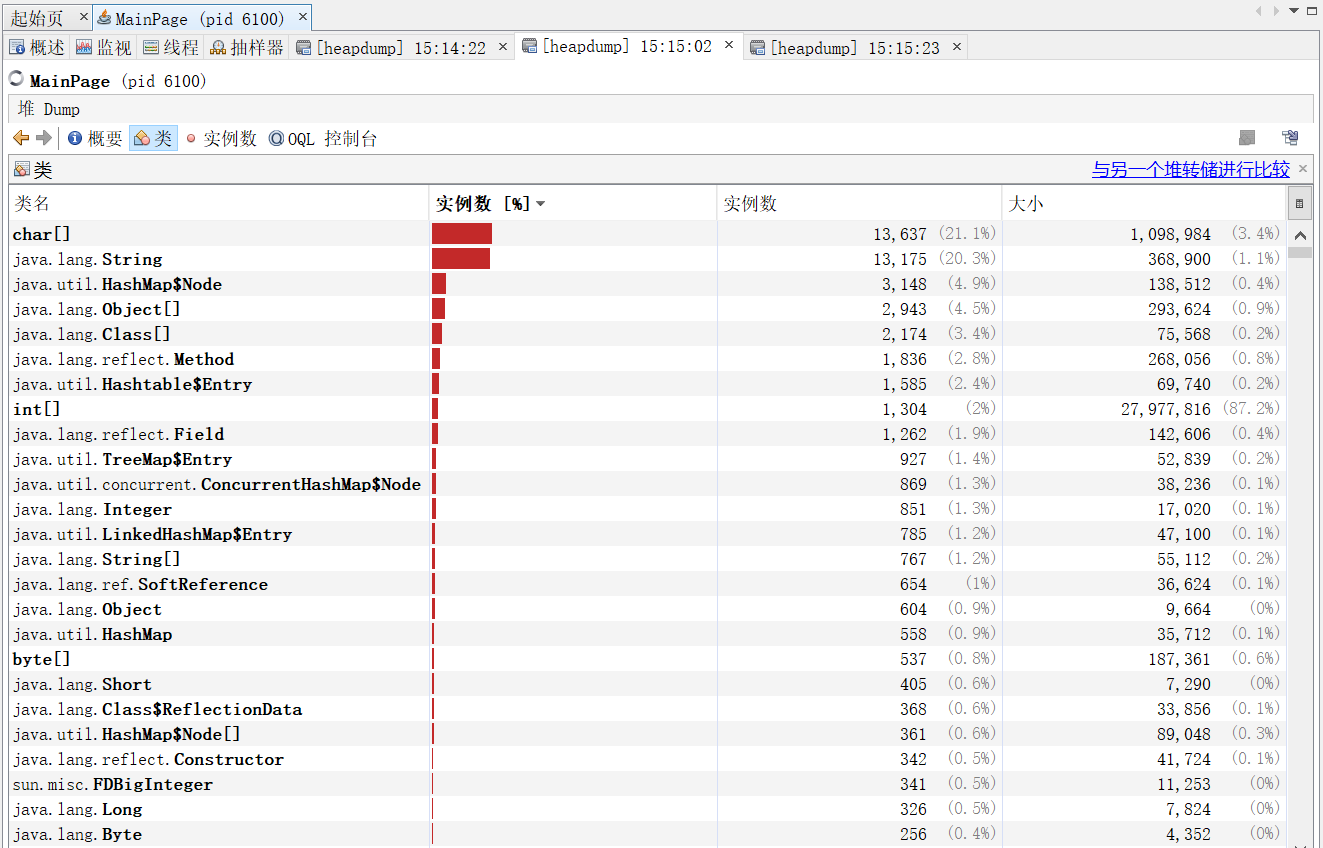
\includegraphics[width=12cm]{/../figures/mm-2-2}
\caption{查询十次桥接词时堆情况}
\label{fig:mm-2-2}
\end{figure}

\begin{figure}
\centering
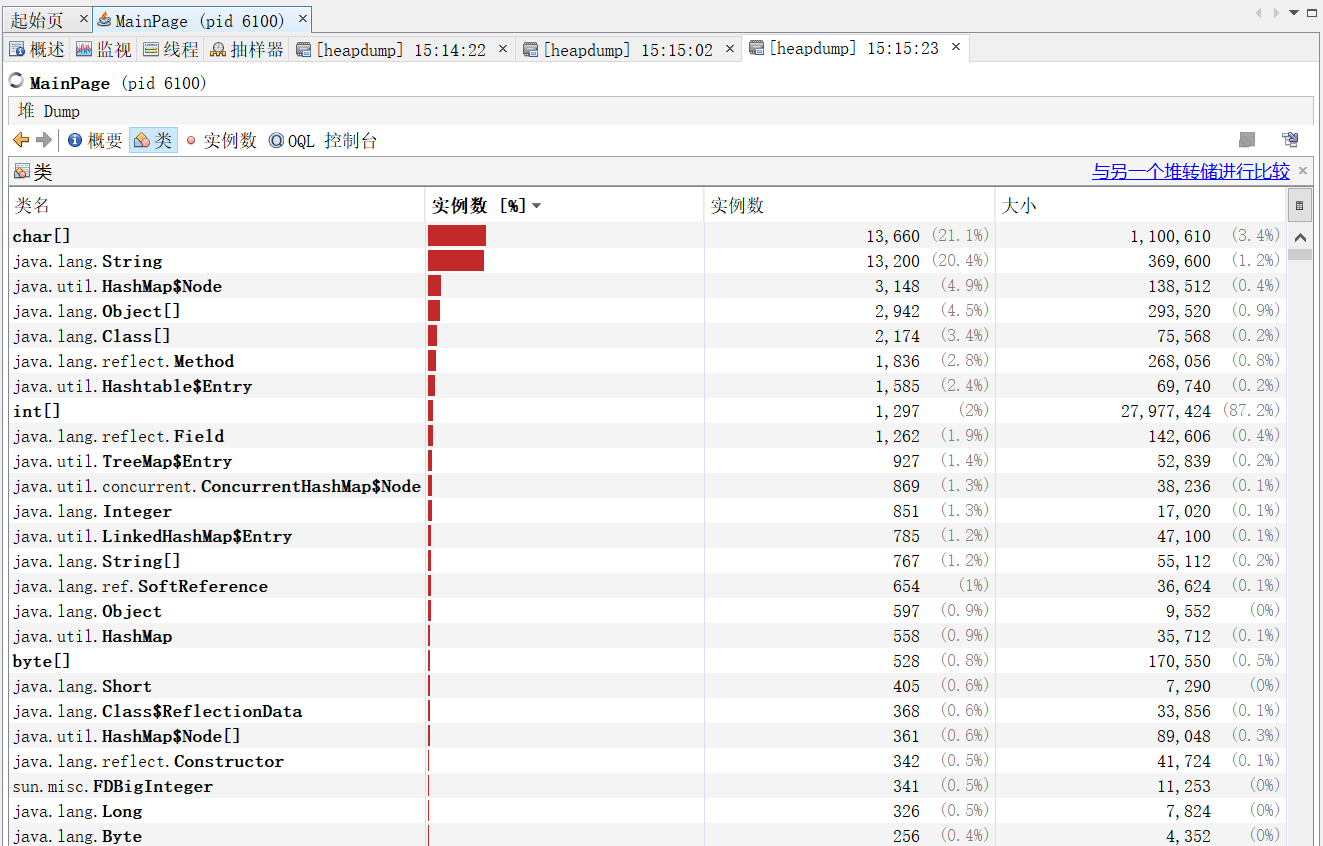
\includegraphics[width=12cm]{/../figures/mm-2-3}
\caption{查询二十次桥接词时堆情况}
\label{fig:mm-2-3}
\end{figure}

\begin{figure}
\centering
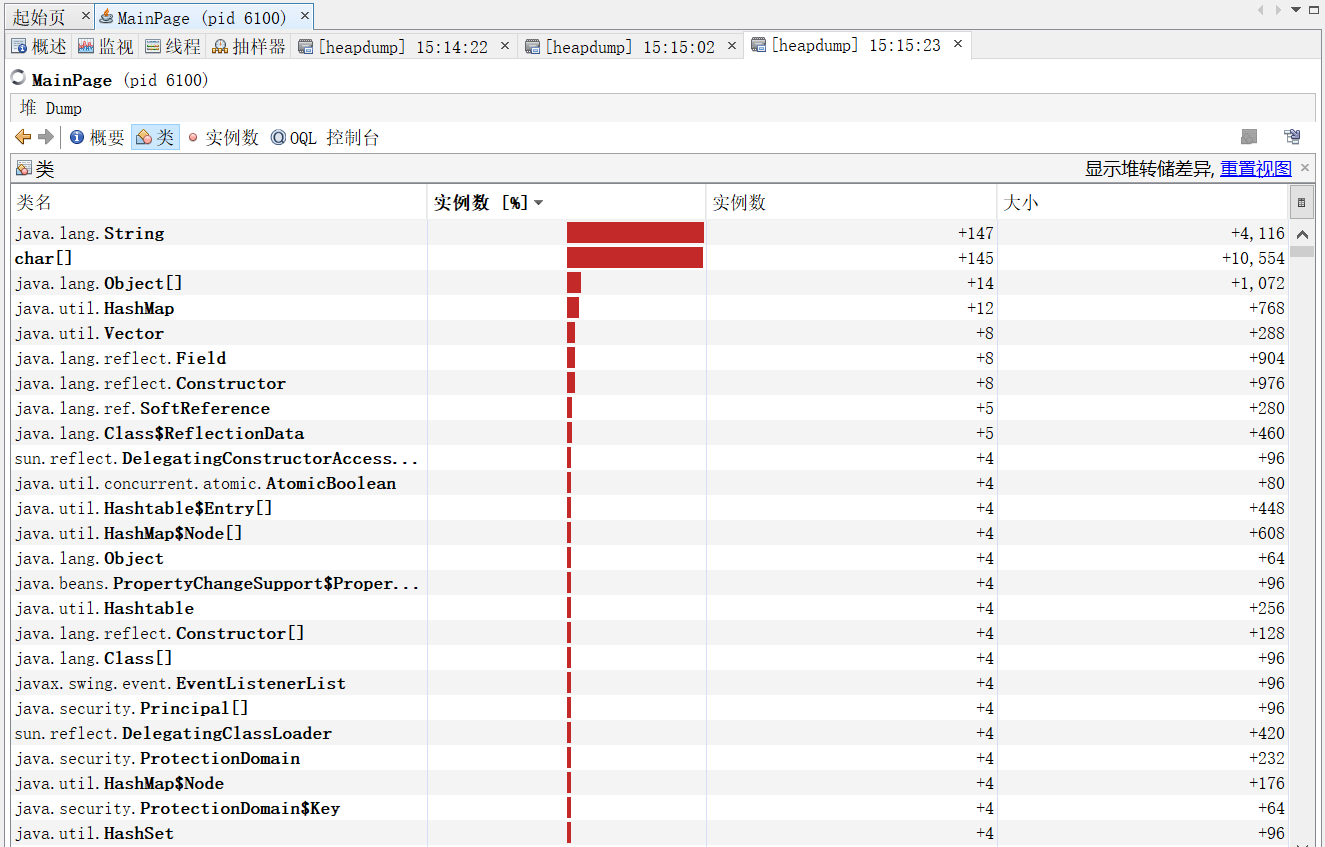
\includegraphics[width=12cm]{/../figures/mm-2-4}
\caption{查询一次与查询二十次堆比较}
\label{fig:mm-2-4}
\end{figure}

由图\ref{fig:mm-2-1},图\ref{fig:mm-2-2},图\ref{fig:mm-2-3},每次记录数据时主要占用堆空间的类同样为char[]以及java.lang.String。同样的,从图\ref{fig:mm-2-1}到图\ref{fig:mm-2-3}的变化中可以看出,每次记录数据时占用堆空间较多的类的实例数以及大小并没有发生较大的改变。由查询二十次桥接词与查询一次桥接词时堆的比较可见看出,char[]的实例数增加了1\%,java.lang.String的实例数增加了1\%,HashMap\$Node的实例数增加了0.3\%,基本可视作没有发生变化,与无内存泄漏时的预期基本一致,因此可以推断出在查询桥接词时未发生内存泄漏。

\BiSubsection{根据桥接词生成新文本}{}
在根据桥接词生成新文本的功能中,我们主要测试多次根据桥接词生成新文本时是否会出现内存泄漏的情况。
测试方法为读入Lab1测试数据中“读取并生成有向图”部分的文件数据,然后在此有向图上进行一次,十次,二十次对同一句子(采用Lab1验收时的句子)来根据桥接词生成新文本,由此分析是否在由桥接词生成新文本的过程中发生了内存泄漏。其中,每次记录堆的数据占用情况前都进行垃圾回收。
由于程序每次完成由桥接词生成新文本之后通过弹出对话框的方式显示生成的文本,关闭对话框后查询结果即消失,因此若无内存泄漏,则可预计所有类的堆占用情况皆不会发生较大的改变。

第一,二,三次记录的数据分别见图\ref{fig:mm-3-1},图\ref{fig:mm-3-2},图\ref{fig:mm-3-3}。执行二十次由桥接词生成新文本与执行一次由桥接词生成新文本时记录的数据的差异比较见图\ref{fig:mm-2-4}。

\begin{figure}
\centering
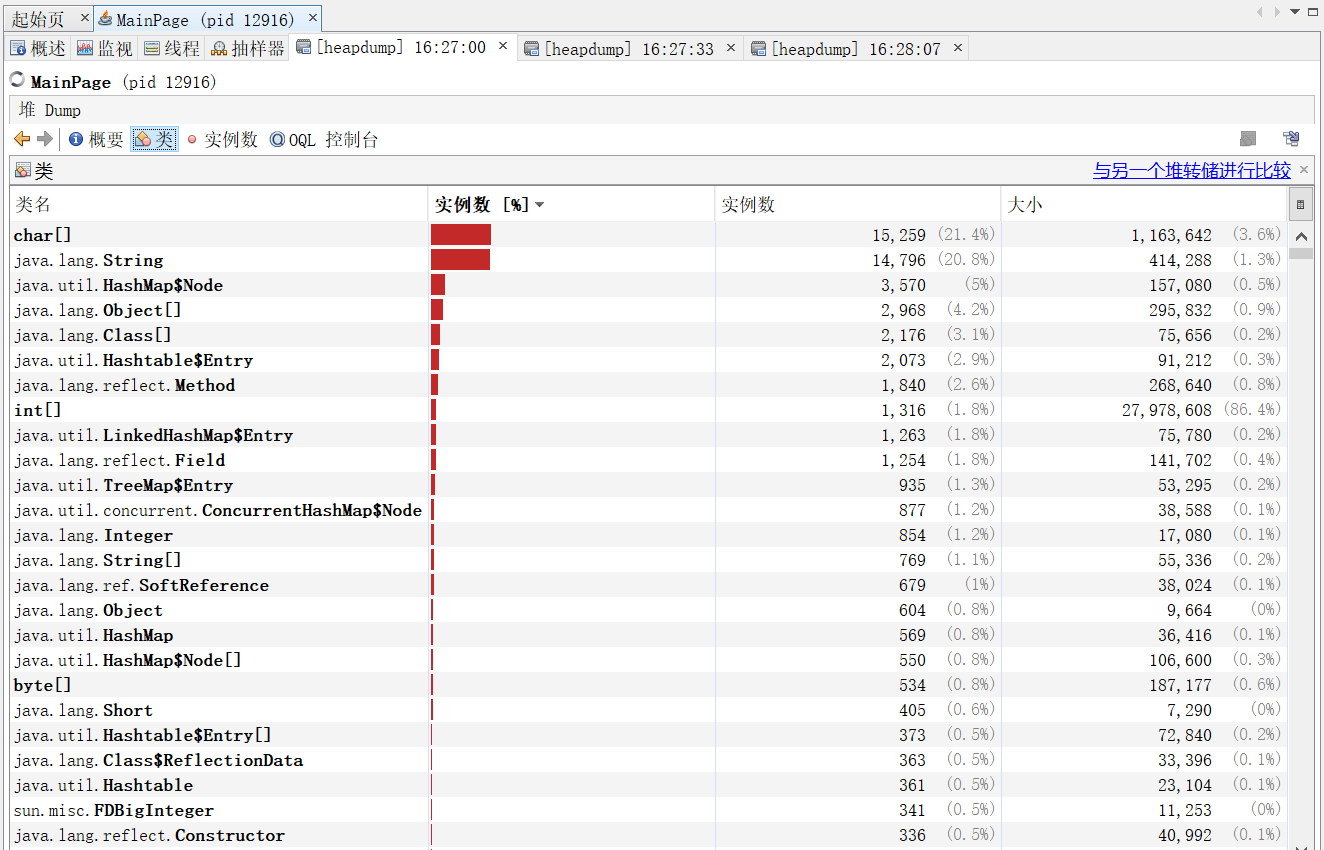
\includegraphics[width=12cm]{/../figures/mm-3-1}
\caption{执行一次时堆情况}
\label{fig:mm-3-1}
\end{figure}

\begin{figure}
\centering
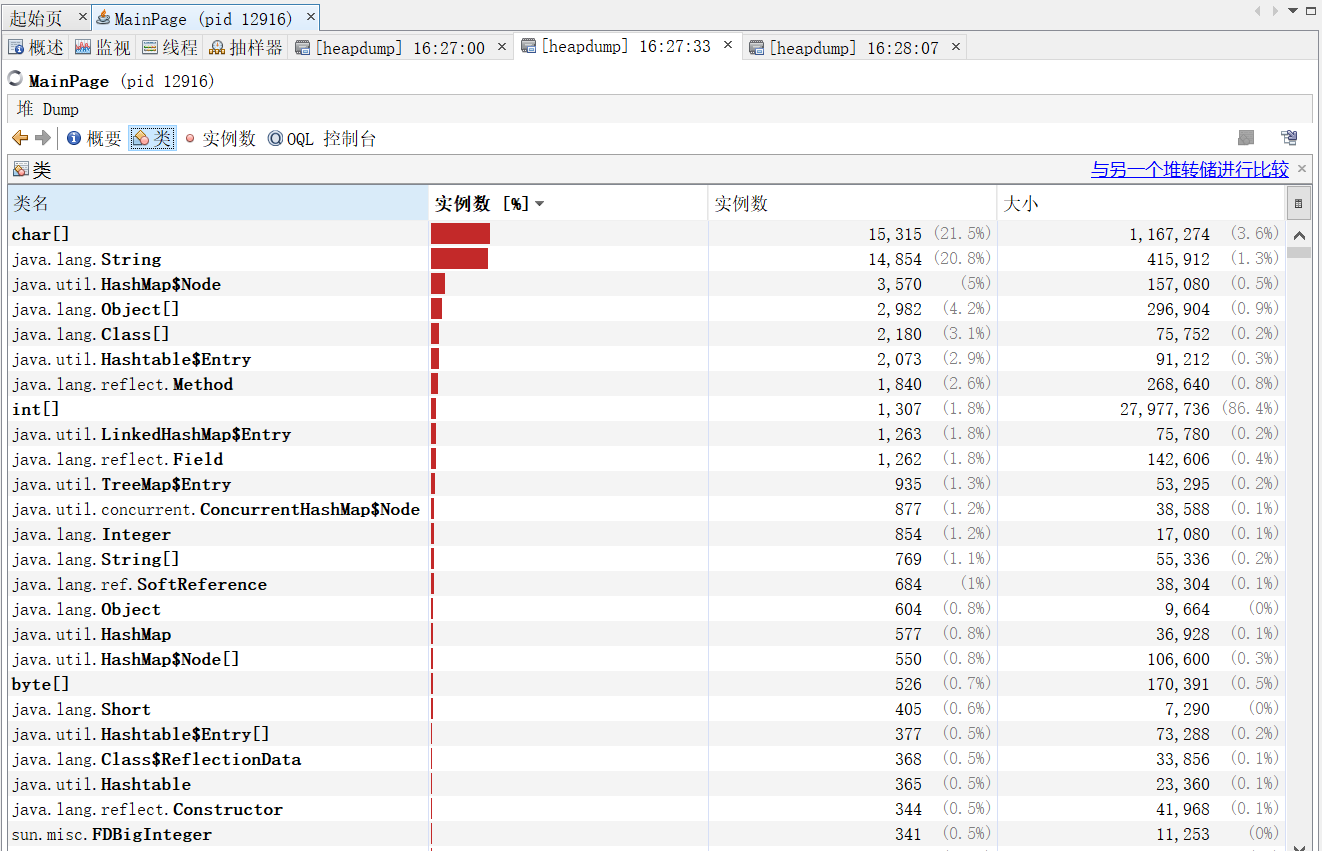
\includegraphics[width=12cm]{/../figures/mm-3-2}
\caption{执行十次时堆情况}
\label{fig:mm-3-2}
\end{figure}

\begin{figure}
\centering
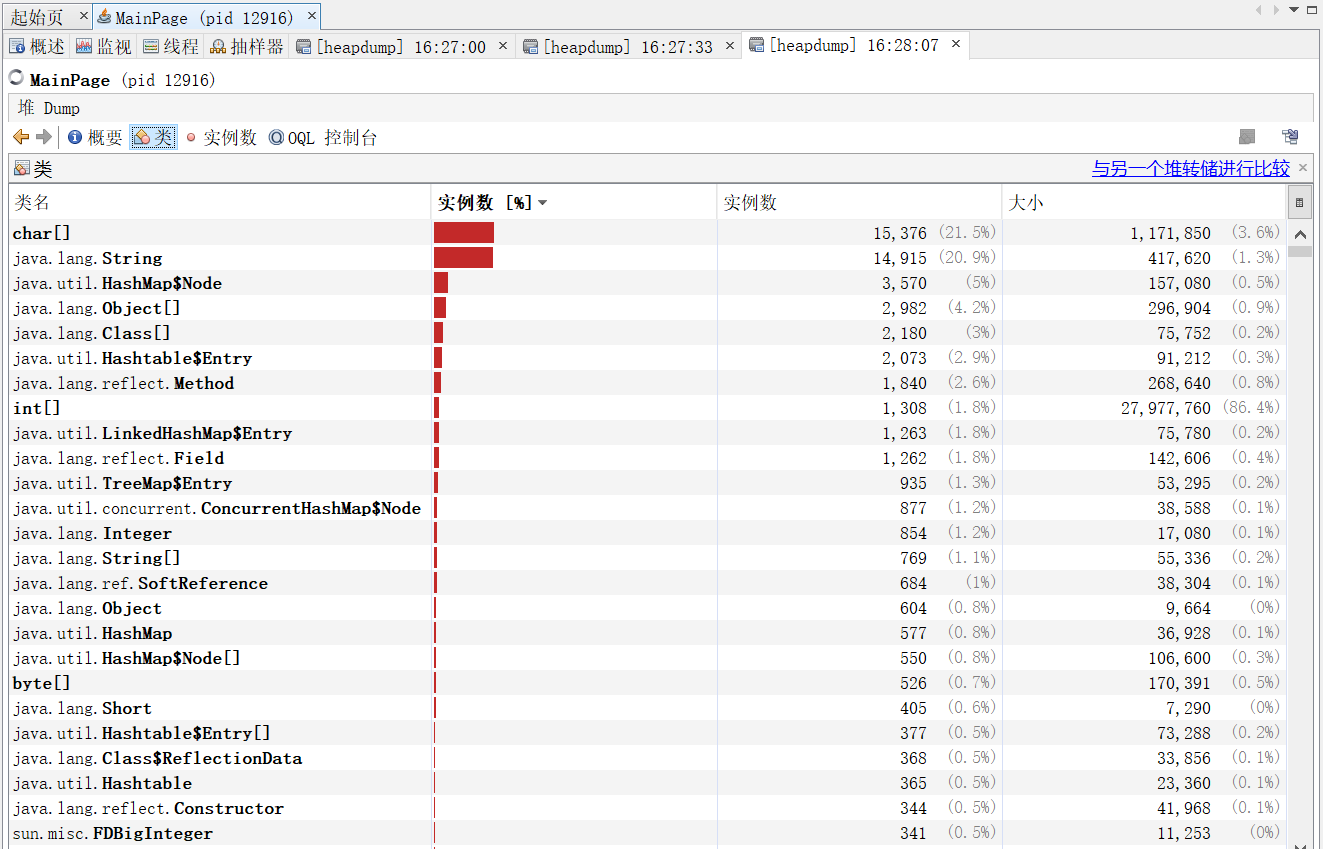
\includegraphics[width=12cm]{/../figures/mm-3-3}
\caption{执行二十次时堆情况}
\label{fig:mm-3-3}
\end{figure}

\begin{figure}
\centering
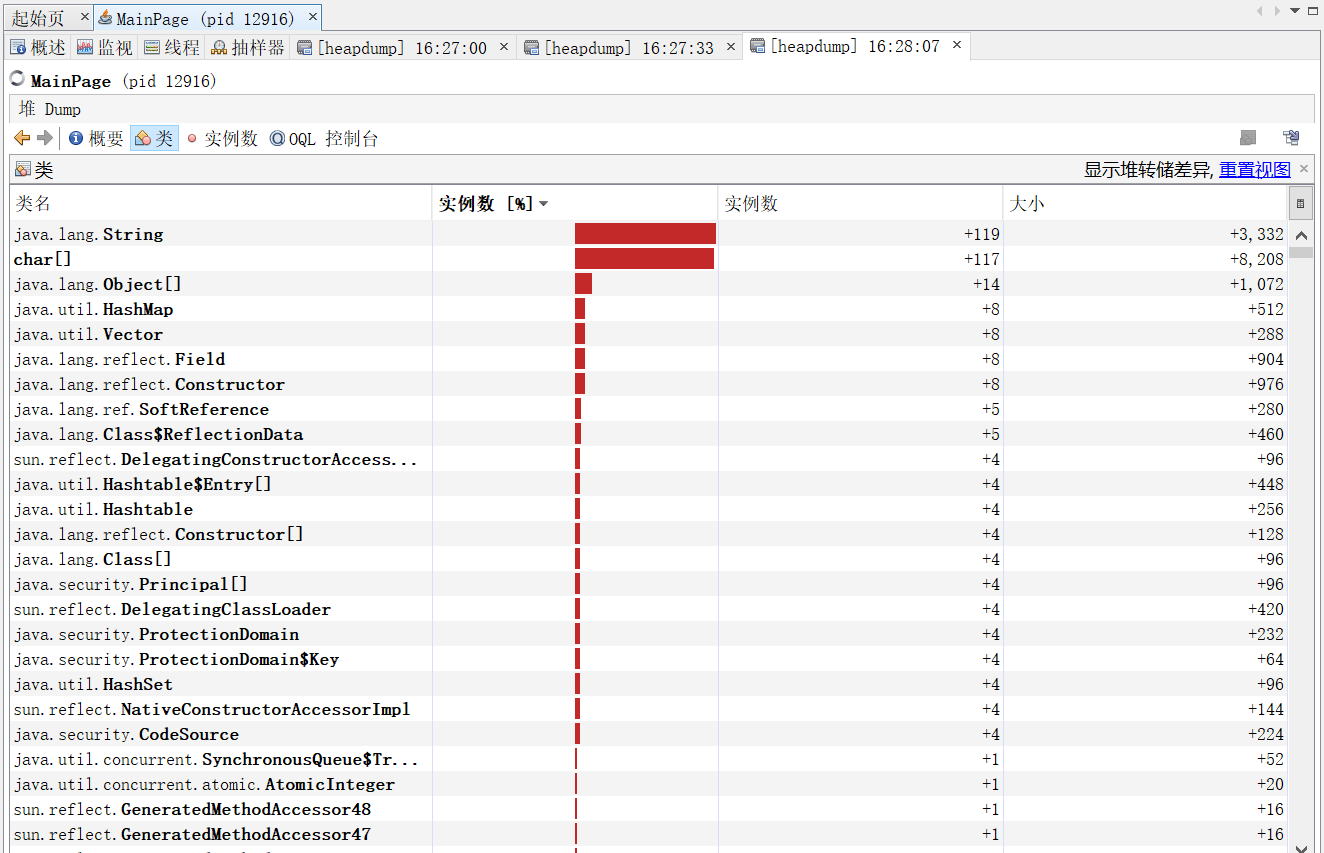
\includegraphics[width=12cm]{/../figures/mm-3-4}
\caption{执行一次与执行二十次堆比较}
\label{fig:mm-3-4}
\end{figure}

由图\ref{fig:mm-3-1},图\ref{fig:mm-3-2},图\ref{fig:mm-3-3},每次记录数据时主要占用堆空间的类同样为char[]以及java.lang.String。同样的,从图\ref{fig:mm-3-1}到图\ref{fig:mm-3-3}的变化中可以看出,每次记录数据时占用堆空间较多的类的实例数以及大小并没有发生较大的改变。由执行二十次由桥接词生成新文本与执行一次由桥接词生成新文本时堆的比较可见看出,char[]的实例数增加了0.7\%,java.lang.String的实例数增加了0.7\%,HashMap\$Node的实例数增加了0\%,因此各个类的实例数基本可视作没有发生变化,与无内存泄漏时的预期基本一致,因此可以推断出在由桥接词生成新文本时未发生内存泄漏。

\BiSubsection{计算两个单词之间的最短路径}{}
在计算两个单词之间的最短路径的功能中,我们主要测试多次计算同一节点的单源最短路径时是否会出现内存泄漏的情况。
测试方法为读入Lab1测试数据中“读取并生成有向图”部分的文件数据,然后在此有向图上进行一次,十次,二十次对同一单词来计算单源最短路径,由此分析是否在计算最短路径的过程中发生了内存泄漏。其中,每次记录堆的数据占用情况前都进行垃圾回收。
由于程序每次完成最短路径的计算之后通过弹出对话框的方式显示计算得到的最短路径,关闭对话框后查询结果即消失,因此若无内存泄漏,则可预计所有类的堆占用情况皆不会发生较大的改变。

第一,二,三次记录的数据分别见图\ref{fig:mm-4-1},图\ref{fig:mm-4-2},图\ref{fig:mm-4-3}。执行二十次计算单源最短路径与执行一次计算单源最短路径时记录的数据的差异比较见图\ref{fig:mm-4-4}。

\begin{figure}
\centering
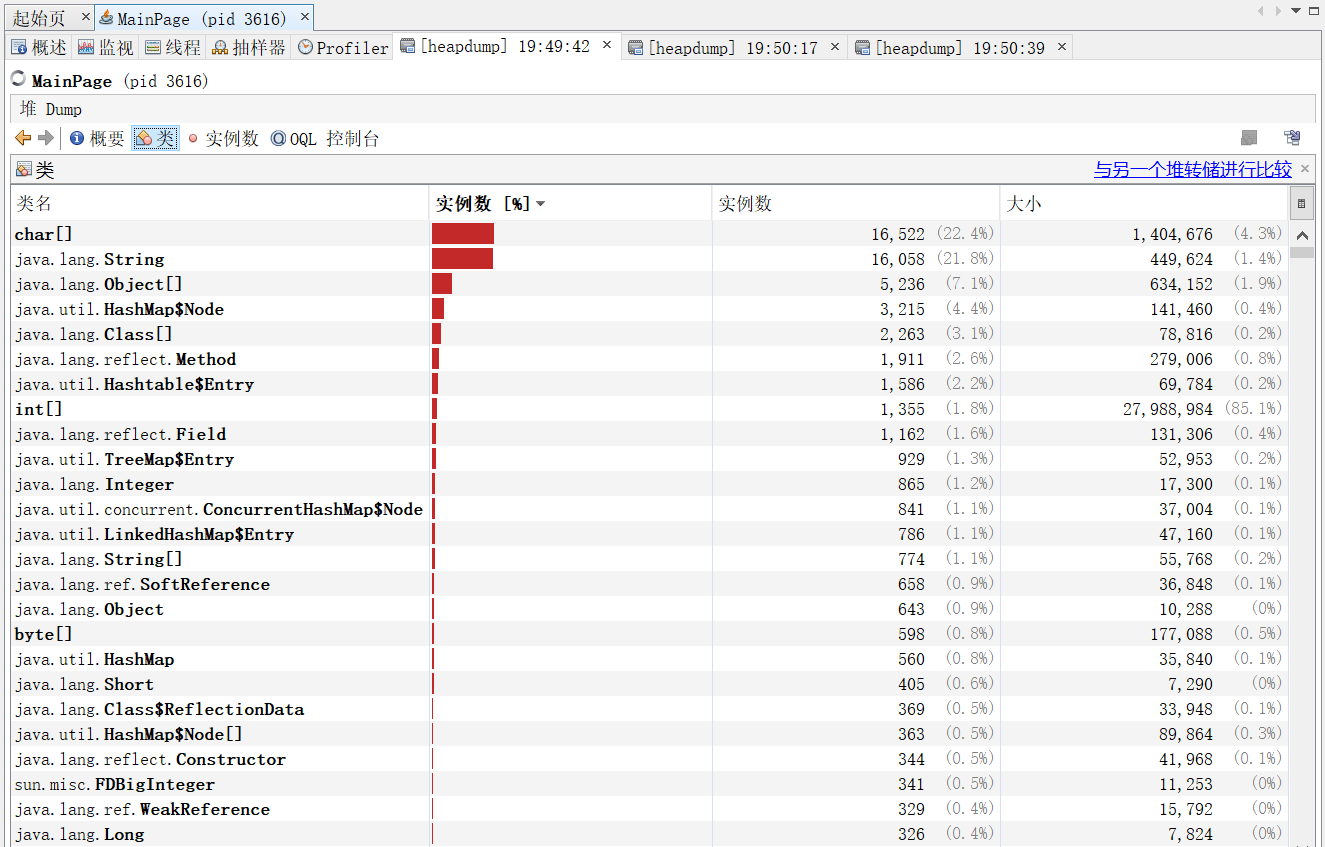
\includegraphics[width=12cm]{/../figures/mm-4-1}
\caption{执行一次时堆情况}
\label{fig:mm-4-1}
\end{figure}

\begin{figure}
\centering
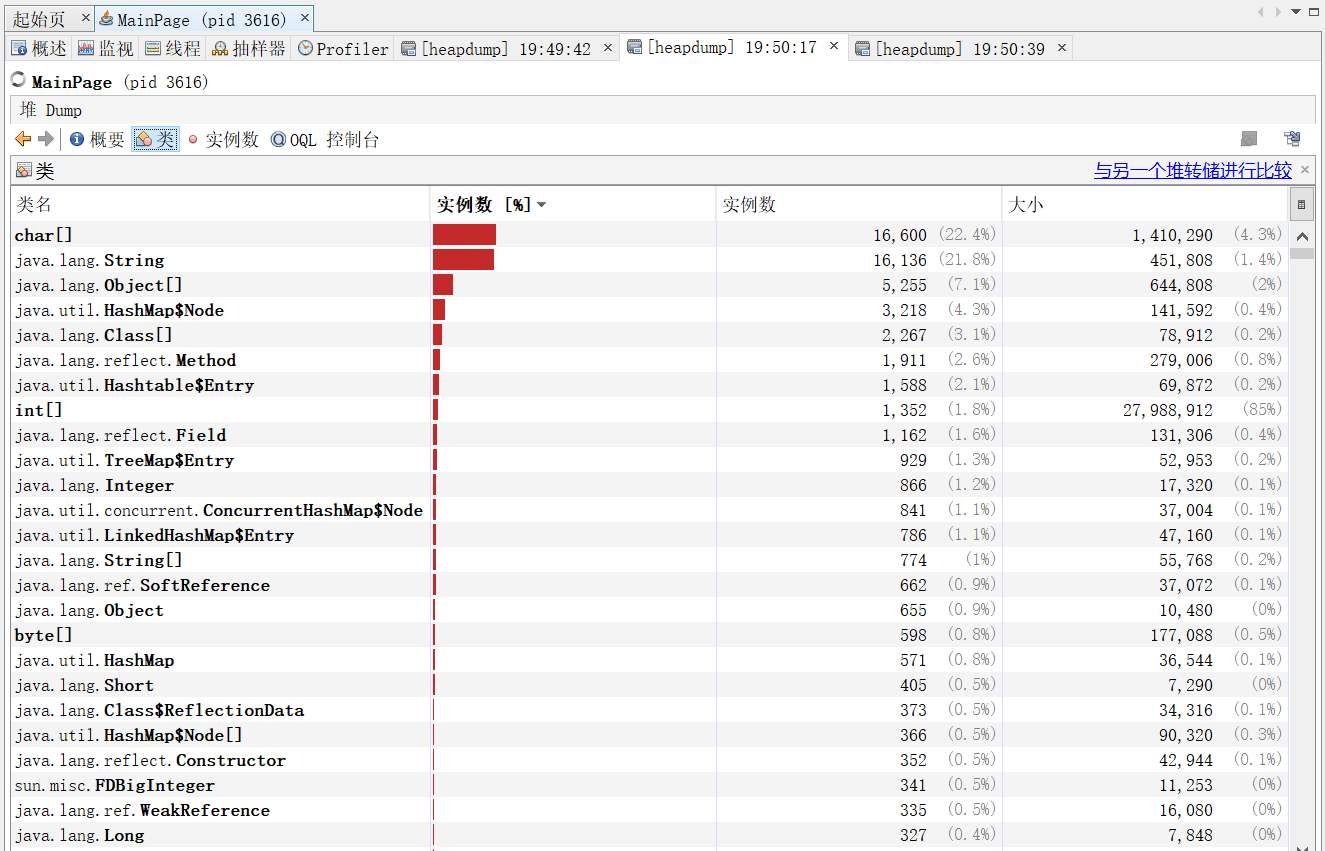
\includegraphics[width=12cm]{/../figures/mm-4-2}
\caption{执行十次时堆情况}
\label{fig:mm-4-2}
\end{figure}

\begin{figure}
\centering
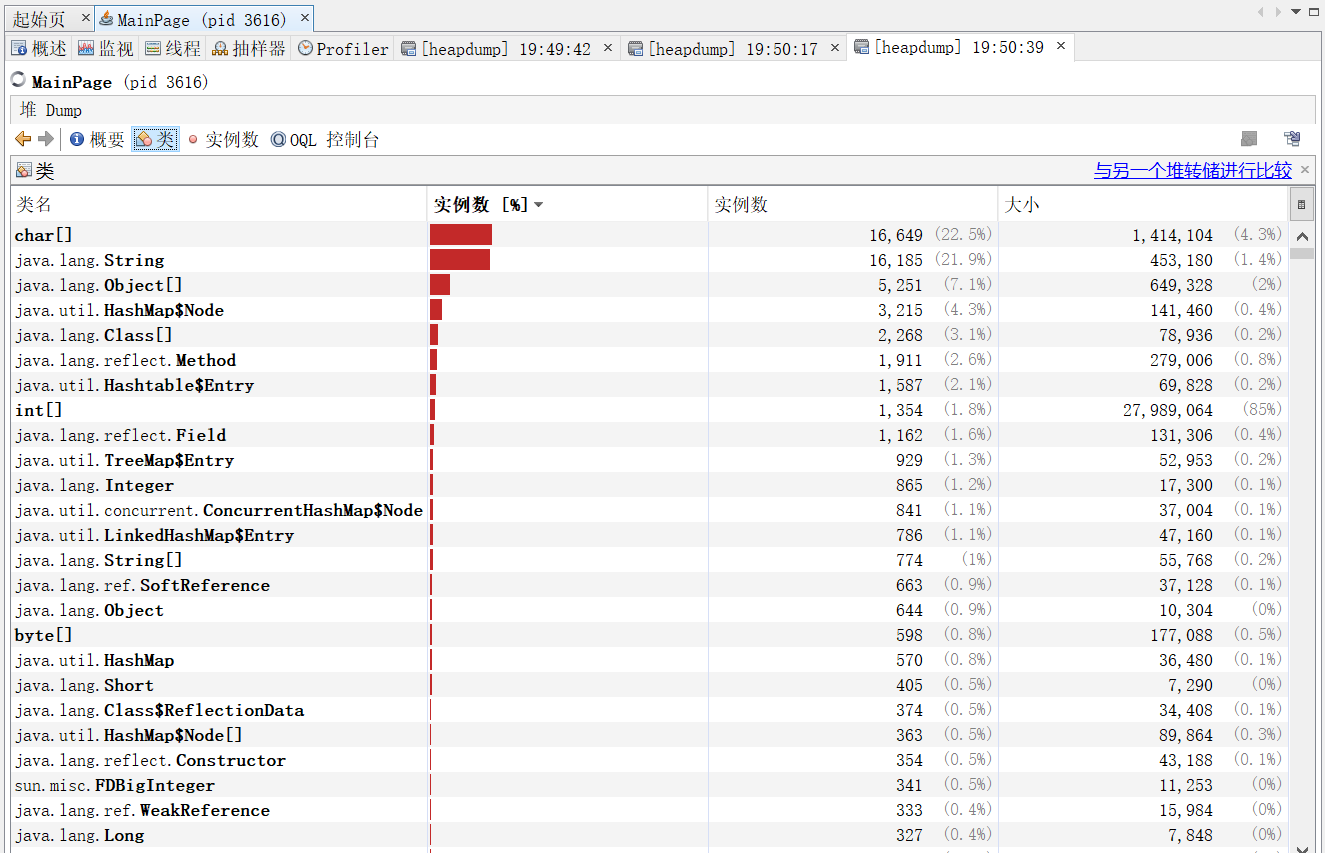
\includegraphics[width=12cm]{/../figures/mm-4-3}
\caption{执行二十次时堆情况}
\label{fig:mm-4-3}
\end{figure}

\begin{figure}
\centering
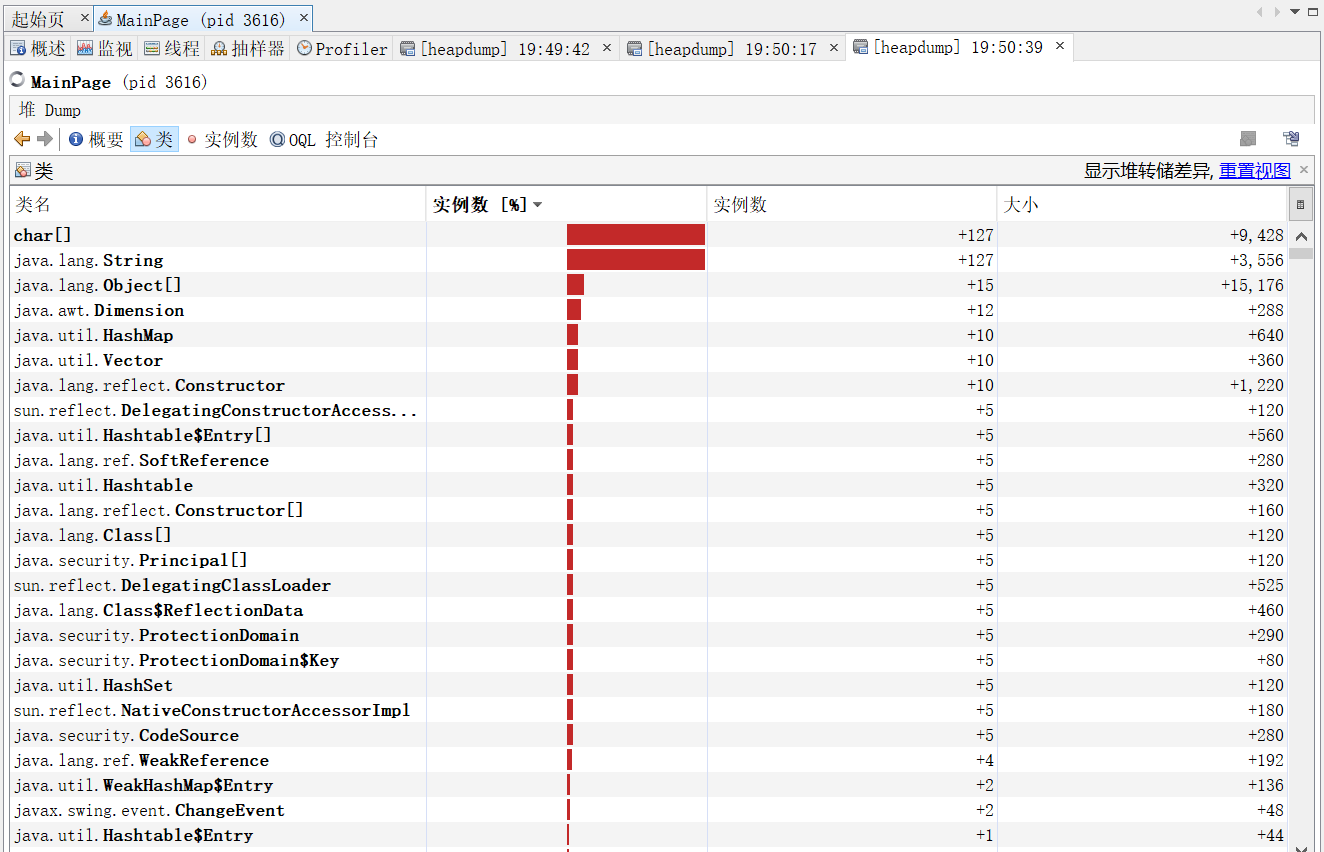
\includegraphics[width=12cm]{/../figures/mm-4-4}
\caption{执行一次与执行二十次堆比较}
\label{fig:mm-4-4}
\end{figure}

由图\ref{fig:mm-4-1},图\ref{fig:mm-4-2},图\ref{fig:mm-4-3}可知,与之前类似的,每次记录数据时主要占用堆空间的类同样为char[]以及java.lang.String。同样的,从图\ref{fig:mm-4-1}到图\ref{fig:mm-4-3}的变化中可以看出,每次记录数据时占用堆空间较多的类的实例数以及大小并没有发生较大的改变。由执行二十次单源最短路径的计算与执行一次单源最短路径的计算时堆的比较可见看出,char[]的实例数增加了0.7\%,java.lang.String的实例数增加了0.7\%,java.lang.Objtec[]的实例数增加了0.2\%,HashMap\$Node的实例数增加了0.3\%,因此各个类的实例数基本可视作没有发生变化,与无内存泄漏时的预期基本一致,因此可以推断出在计算最短路径时未发生内存泄漏

\BiSubsection{随机游走}{}
在测试随机游走时,我们采用同样的方法测试在随机游走的过程中是否出现了内存泄漏。
测试的方法为读入Lab1测试数据中“读取并生成有向图”部分的文件数据,然后在此有向图上进行一次,十次,二十次随机游走并记录堆的信息,每一次随机游走皆进行到没有节点可以继续游走为止,由此分析是否在计算最短路径的过程中发生了内存泄漏。其中,每次记录堆的数据占用情况前都进行垃圾回收。
由于每一次随机游走之间没有相互关联,GUI中也不保留随机游走的数据,因此在没有发生内存泄漏的前提下,可预计所有类的堆占用情况皆不会发生较大的改变。

第一,二,三次记录的数据分别见图\ref{fig:mm-5-1},图\ref{fig:mm-5-2},图\ref{fig:mm-5-3}。执行二十次随机游走与执行一次随机游走时记录的数据的差异比较见图\ref{fig:mm-5-4}。

\begin{figure}
\centering
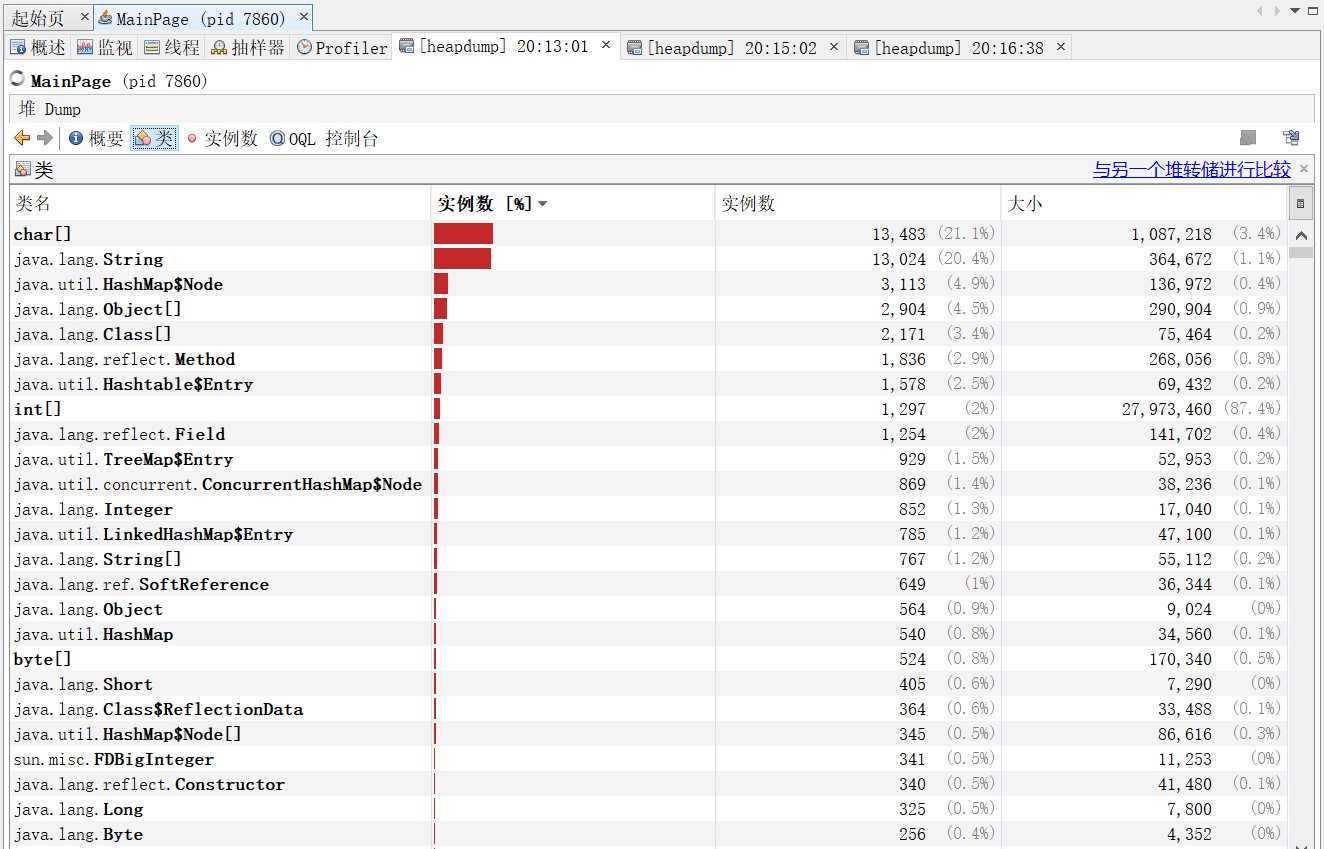
\includegraphics[width=12cm]{/../figures/mm-5-1}
\caption{执行一次时堆情况}
\label{fig:mm-5-1}
\end{figure}

\begin{figure}
\centering
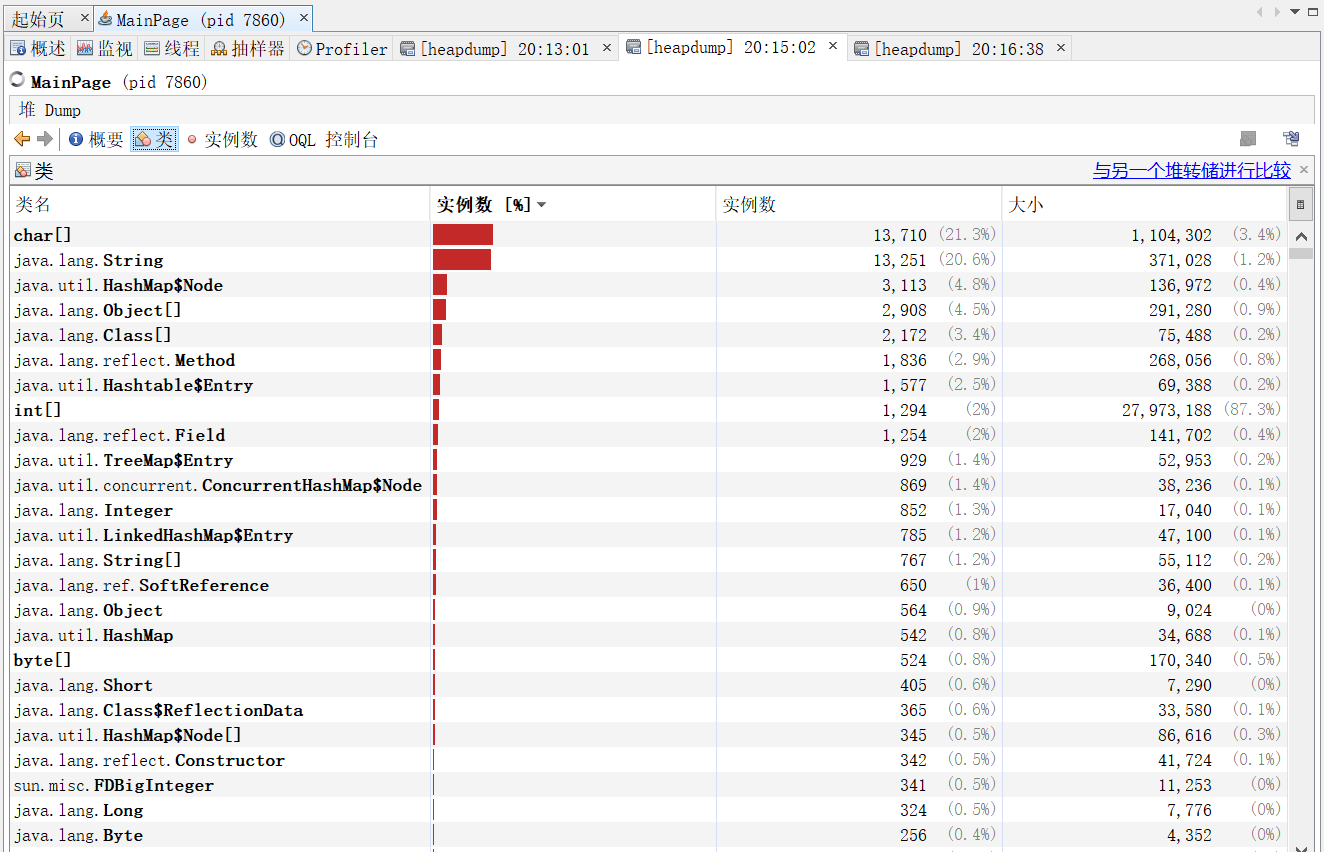
\includegraphics[width=12cm]{/../figures/mm-5-2}
\caption{执行十次时堆情况}
\label{fig:mm-5-2}
\end{figure}

\begin{figure}
\centering
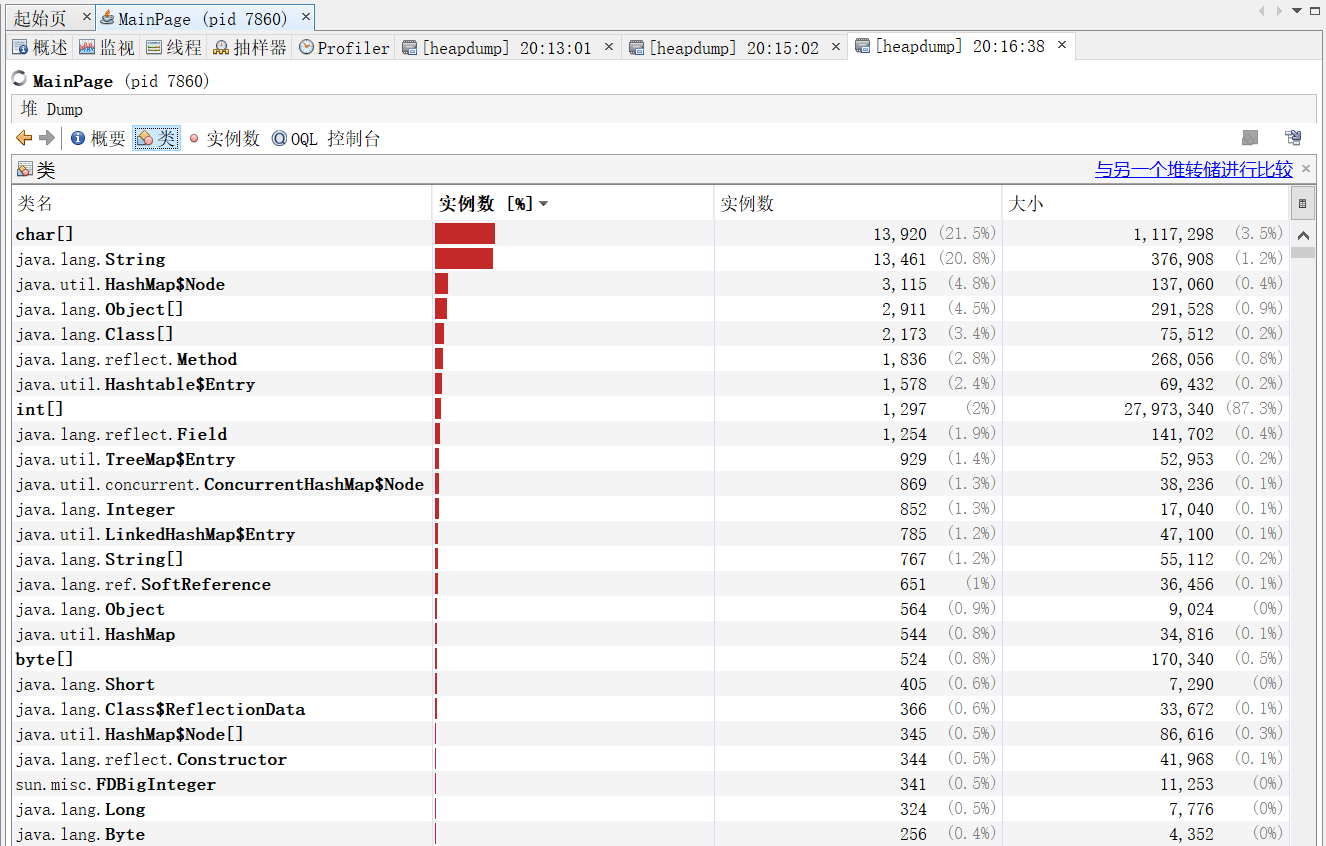
\includegraphics[width=12cm]{/../figures/mm-5-3}
\caption{执行二十次时堆情况}
\label{fig:mm-5-3}
\end{figure}

\begin{figure}
\centering
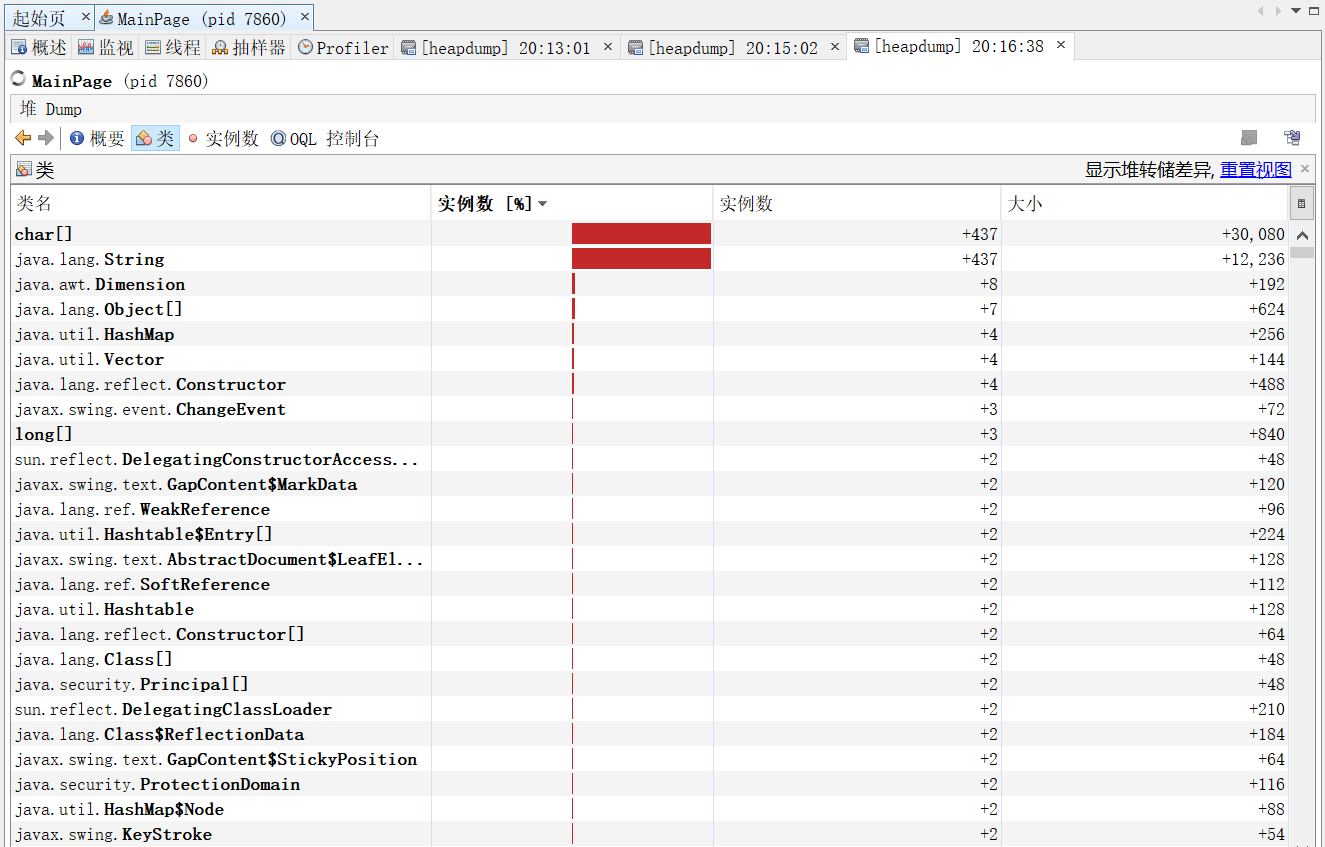
\includegraphics[width=12cm]{/../figures/mm-5-4}
\caption{执行一次与执行二十次堆比较}
\label{fig:mm-5-4}
\end{figure}

由图\ref{fig:mm-5-1},图\ref{fig:mm-5-2},图\ref{fig:mm-5-3}可知,与之前类似的,每次记录数据时主要占用堆空间的类同样为char[]以及java.lang.String。同样的,从图\ref{fig:mm-5-1}到图\ref{fig:mm-5-3}的变化中可以看出,每次记录数据时占用堆空间较多的类的实例数以及大小并没有发生较大的改变。由执行二十次随机游走与执行一次随机游走时堆的比较可见看出,char[]的实例数增加了3\%,java.lang.String的实例数增加了3\%,HashMap\$Node的实例数增加了0.06\%,因此各个类的实例数基本可视作没有发生变化,与无内存泄漏时的预期基本一致,因此可以推断出在随机游走时未发生内存泄漏。

最后,值得一提的是,在上述五种功能的分析中,所有的功能的堆信息中占用堆最多的都是char[]以及java.lang.string两个类,并且两个类的实例个数非常相近。这是因此在java.lang.String类中,即有char[]作为其实例变量来存储java.lang.String表示的字符串中的字符,因此任何一个java.lang.String的对象都会有一个char[]变量,故其实例数量相近。

\BiSection{代码改进之后的执行时间统计结果}{}
在本节中将给出代码改进之后的执行时间统计结果。
由使用VisualVM进行耗时分析以及内存分析的结果可知,在不改变GUI框架以及使用GraphViz进行绘图的前提下无法从耗时方面对程序的性能进行优化,也因为没有出现内存泄漏而无法通过消除内存泄漏来改进代码。因此本节中采用的修改后的代码为进行代码review,checkstyle,FindBugs,PMD进行检测与修正后的代码,并不包含利用VisualVM进行代码改进的部分。

对改进代码进行时间测试的方法为:依次执行“生成并展示有向图”,“查询桥接词”,“由桥接词生成新文本”,“计算最短路径”,“随机游走”五个功能,其中“生成并展示有向图”输入数据为Lab1的验收文件,“查询桥接词为”为查询从the到of的桥接词,“由桥接词生成新文本”中的文本为“In the big time, servitization one of the important trends-of the IT world.”,“计算最短路径”为计算单词in的单源最短路径,“随机游走”为游走到没有可选节点为止。测试时分别对每个功能执行时各个函数的耗时利用VisualVM进行记录。

“生成并展示有向图”耗时图像为图\ref{fig:new-time-1},“查询桥接词”耗时图像为图\ref{fig:new-time-2},“由桥接词生成新文本”耗时图像为图\ref{fig:new-time-3},“计算最短路径”耗时图像为图\ref{fig:new-time-4},“随机游走”耗时图像为图\ref{fig:new-time-5}。

\begin{figure}
\centering
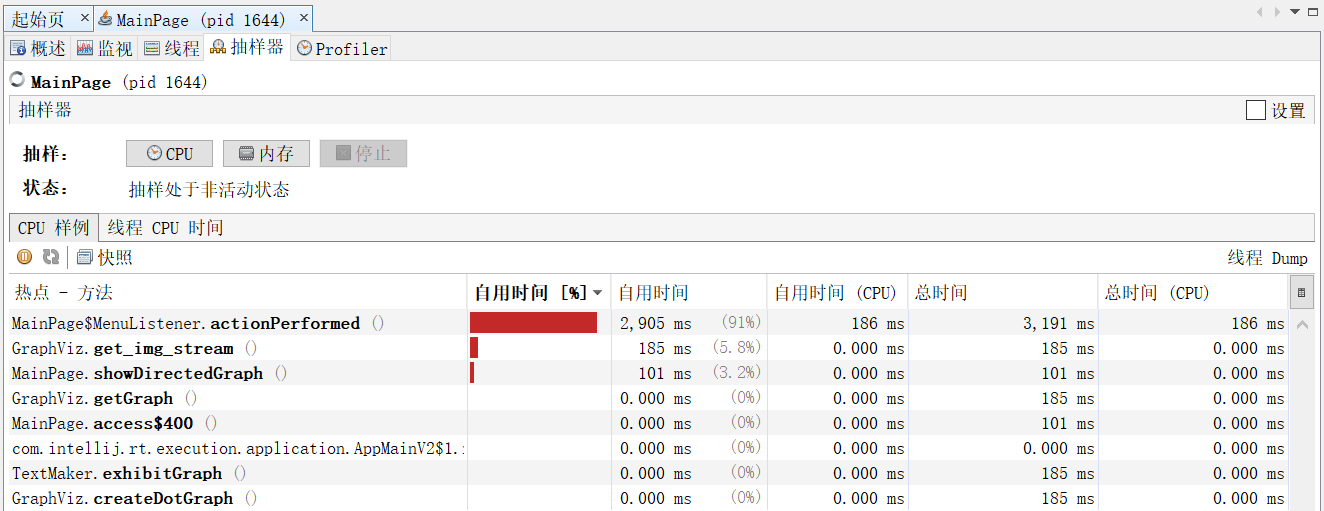
\includegraphics[width=12cm]{/../figures/new-time-1}
\caption{生成并展示有向图耗时}
\label{fig:new-time-1}
\end{figure}

\begin{figure}
\centering
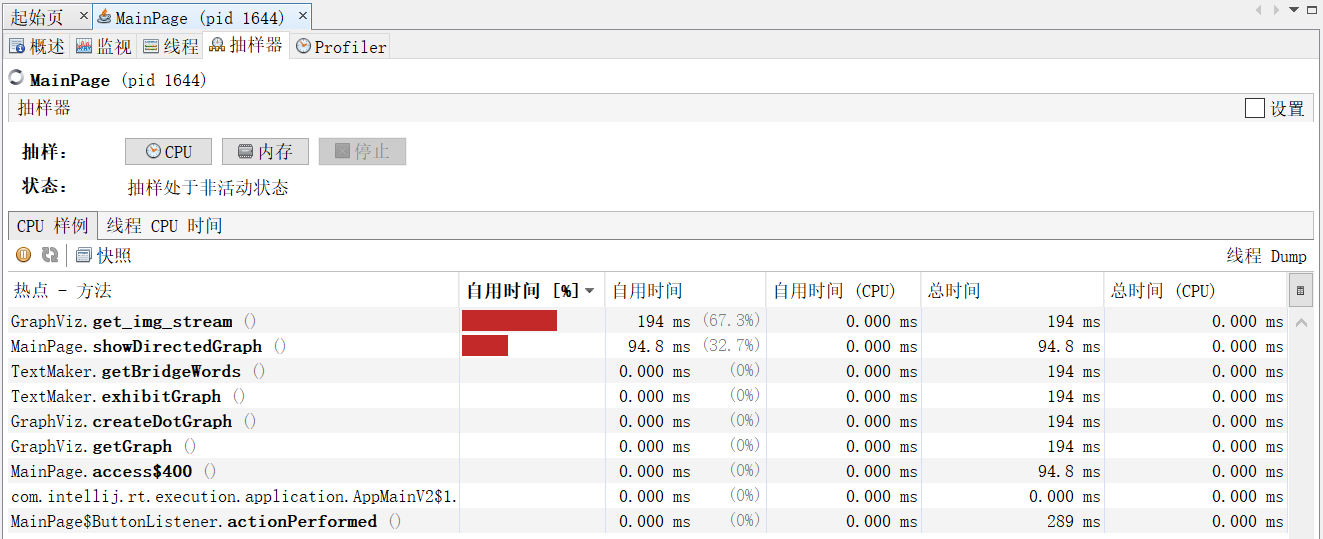
\includegraphics[width=12cm]{/../figures/new-time-2}
\caption{查询桥接词耗时}
\label{fig:new-time-2}
\end{figure}

\begin{figure}
\centering
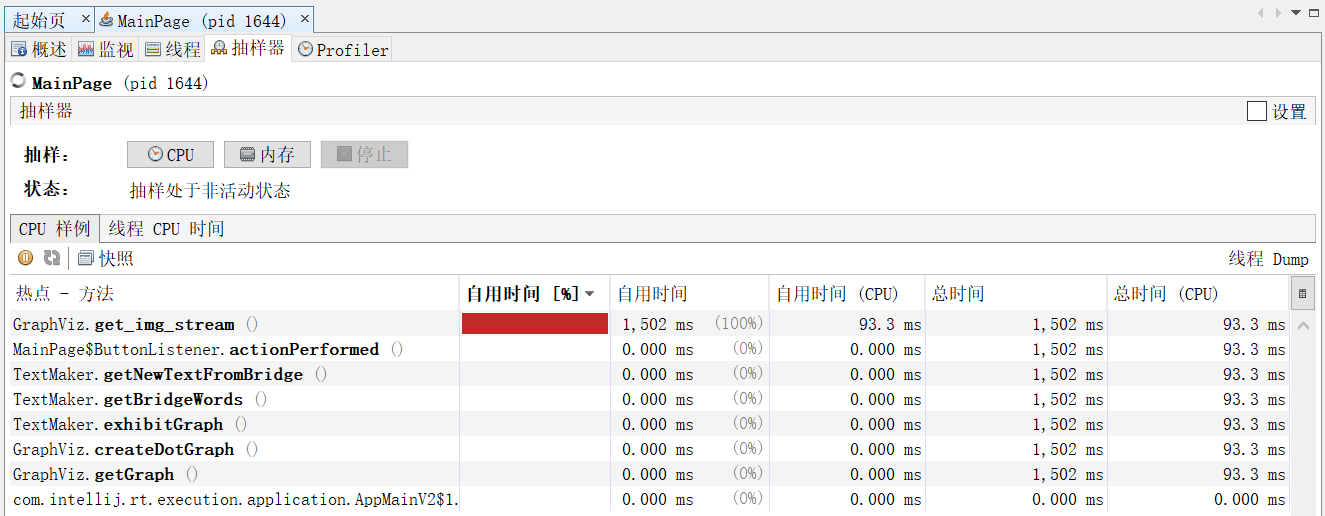
\includegraphics[width=12cm]{/../figures/new-time-3}
\caption{由桥接词生成新文本耗时}
\label{fig:new-time-3}
\end{figure}

\begin{figure}
\centering
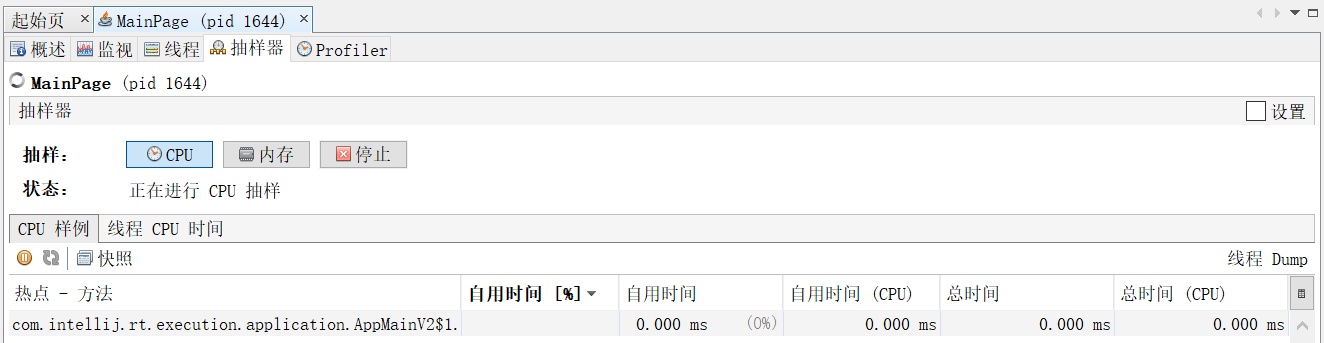
\includegraphics[width=12cm]{/../figures/new-time-4}
\caption{计算最短路径耗时}
\label{fig:new-time-4}
\end{figure}

\begin{figure}
\centering
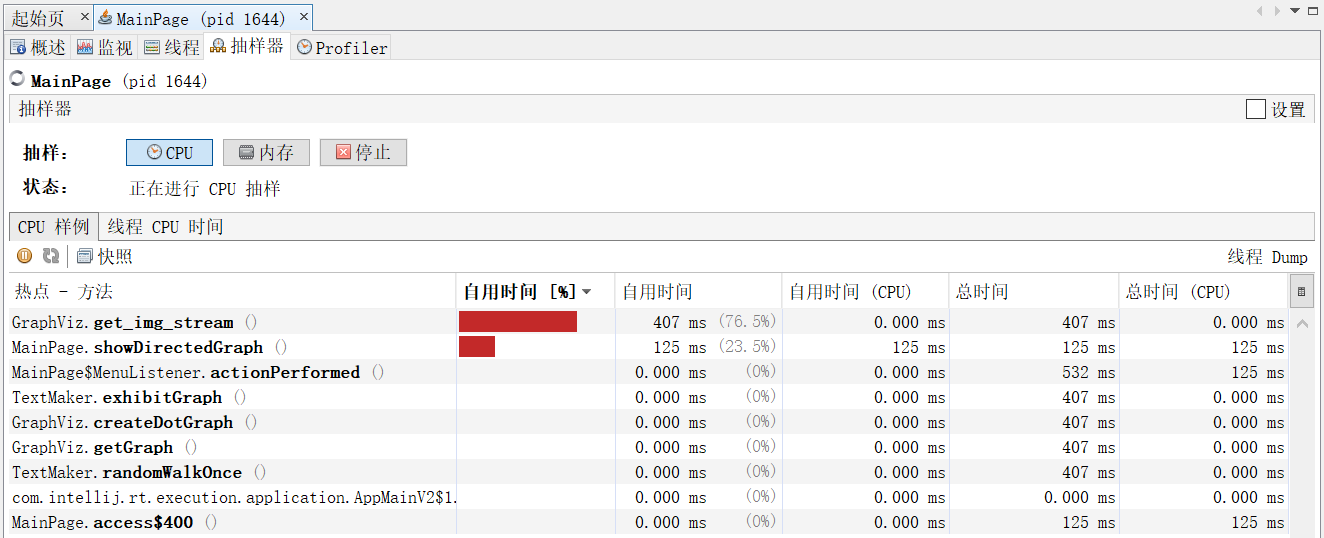
\includegraphics[width=12cm]{/../figures/new-time-5}
\caption{随机游走耗时}
\label{fig:new-time-5}
\end{figure}

\BiSection{代码改进之后的内存占用统计结果}{}
在本节中将给出代码改进之后的内存占用统计结果。
与上一节相同,本节中采用的修改后的代码为进行代码review,checkstyle,FindBugs,PMD进行检测与修正后的代码,并不包含利用VisualVM进行代码改进的部分。

对改进代码进行内存测试的方法为:依次执行“生成并展示有向图”,“查询桥接词”,“由桥接词生成新文本”,“计算最短路径”,“随机游走”五个功能,其中“生成并展示有向图”输入数据为Lab1的验收文件,“查询桥接词为”为查询从the到of的桥接词,“由桥接词生成新文本”中的文本为“In the big time, servitization one of the important trends-of the IT world.”,“计算最短路径”为计算单词in的单源最短路径,“随机游走”为游走到没有可选节点为止。测试时分别对每个功能执行时的堆使用情况利用VisualVM进行记录。

“生成并展示有向图”的堆使用情况图像为图\ref{fig:new-mm-1},“查询桥接词”的堆使用情况图像为图\ref{fig:new-mm-2},“由桥接词生成新文本”的堆使用图像为图\ref{fig:new-mm-3},“计算最短路径”的堆使用图像为图\ref{fig:new-mm-4},“随机游走”的堆使用图像为图\ref{fig:new-mm-5}。

\begin{figure}
\centering
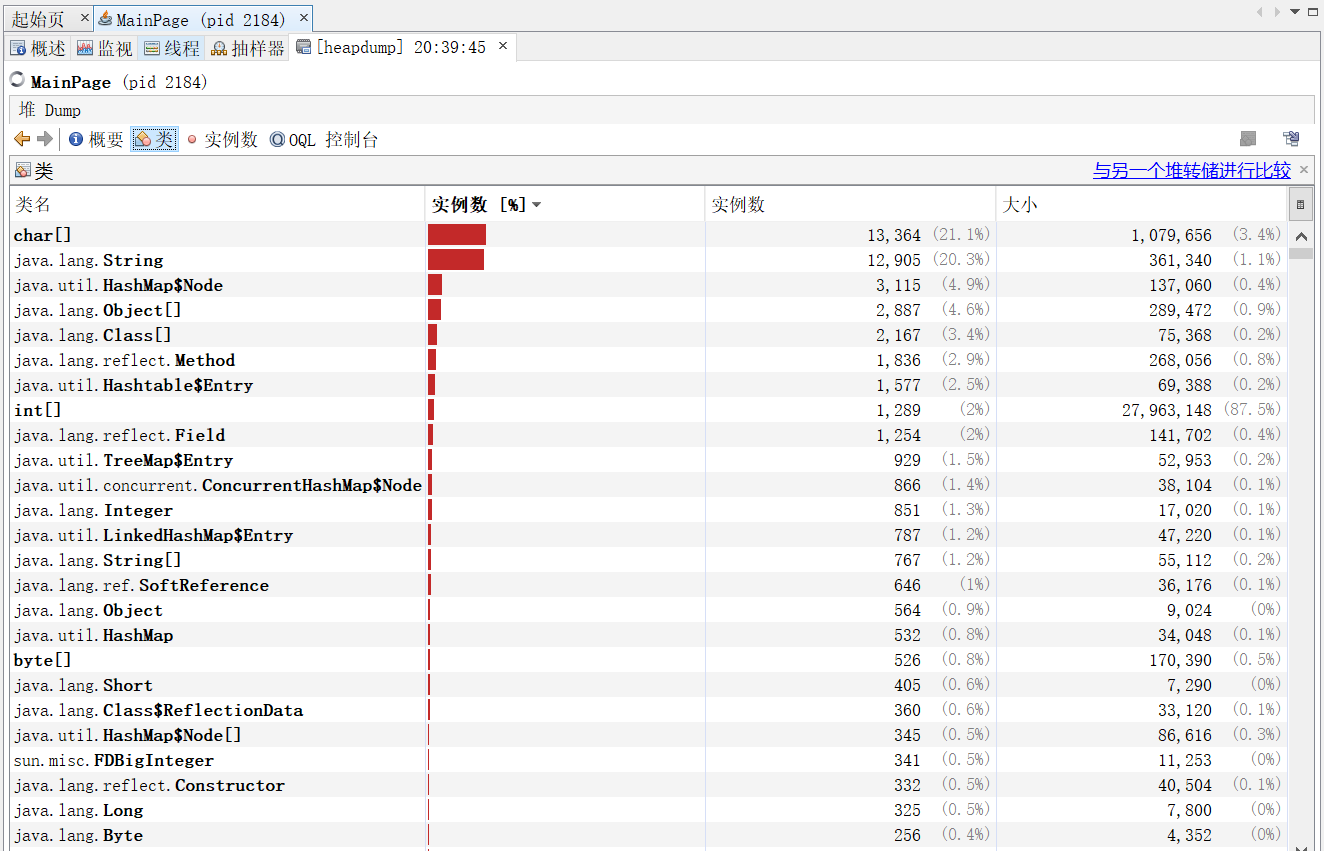
\includegraphics[width=12cm]{/../figures/new-mm-1}
\caption{生成并展示有向图的堆使用}
\label{fig:new-mm-1}
\end{figure}

\begin{figure}
\centering
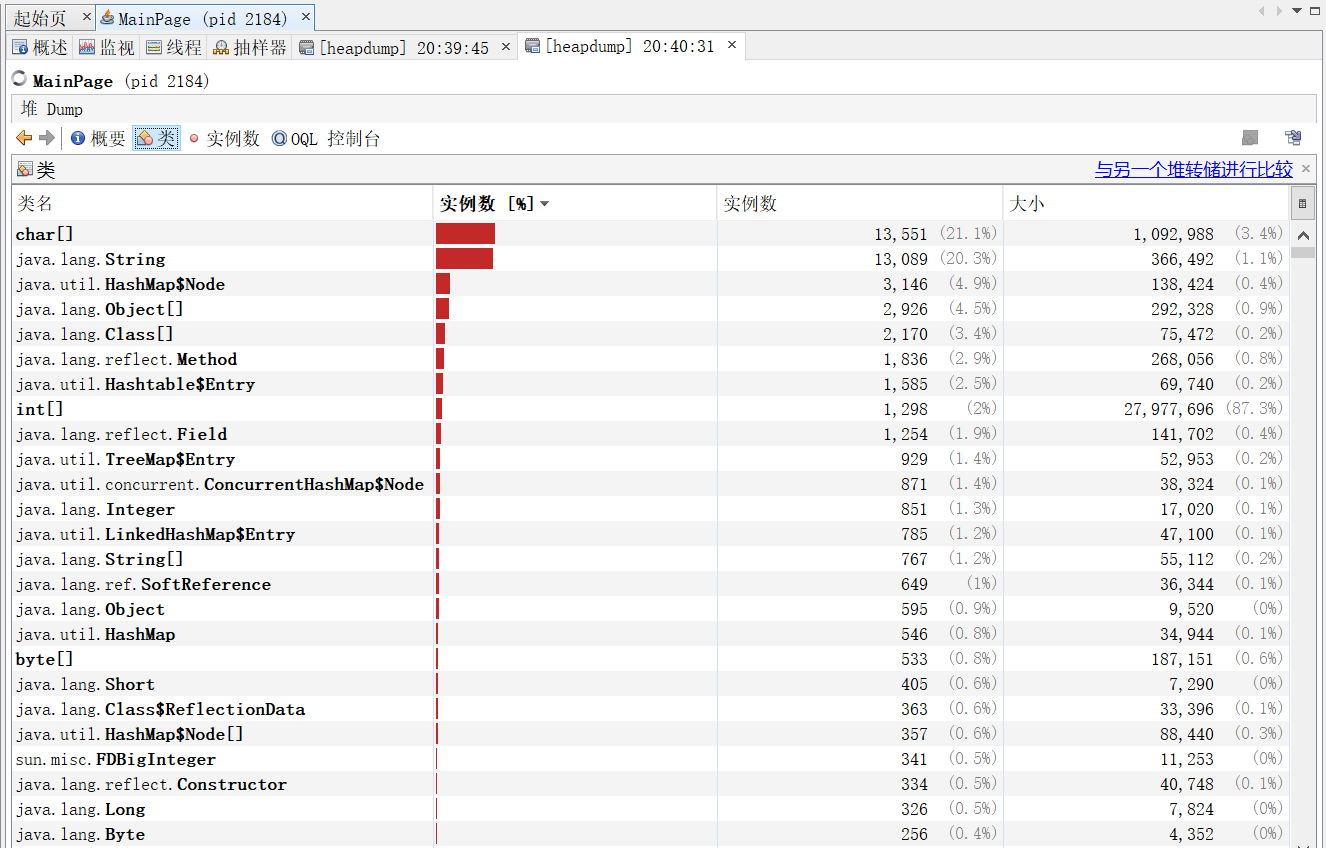
\includegraphics[width=12cm]{/../figures/new-mm-2}
\caption{查询桥接词的堆使用}
\label{fig:new-mm-2}
\end{figure}

\begin{figure}
\centering
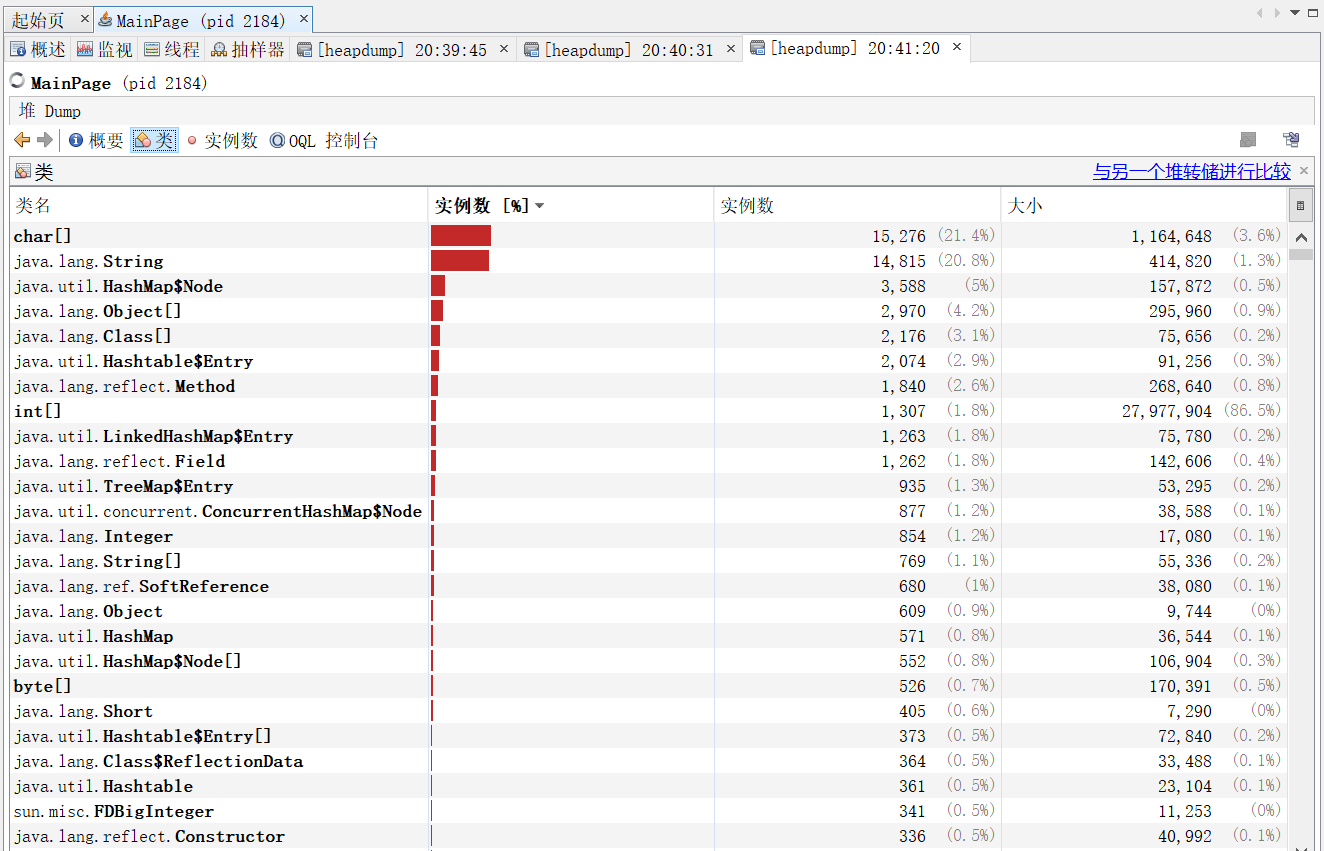
\includegraphics[width=12cm]{/../figures/new-mm-3}
\caption{由桥接词生成新文本的堆使用}
\label{fig:new-mm-3}
\end{figure}

\begin{figure}
\centering
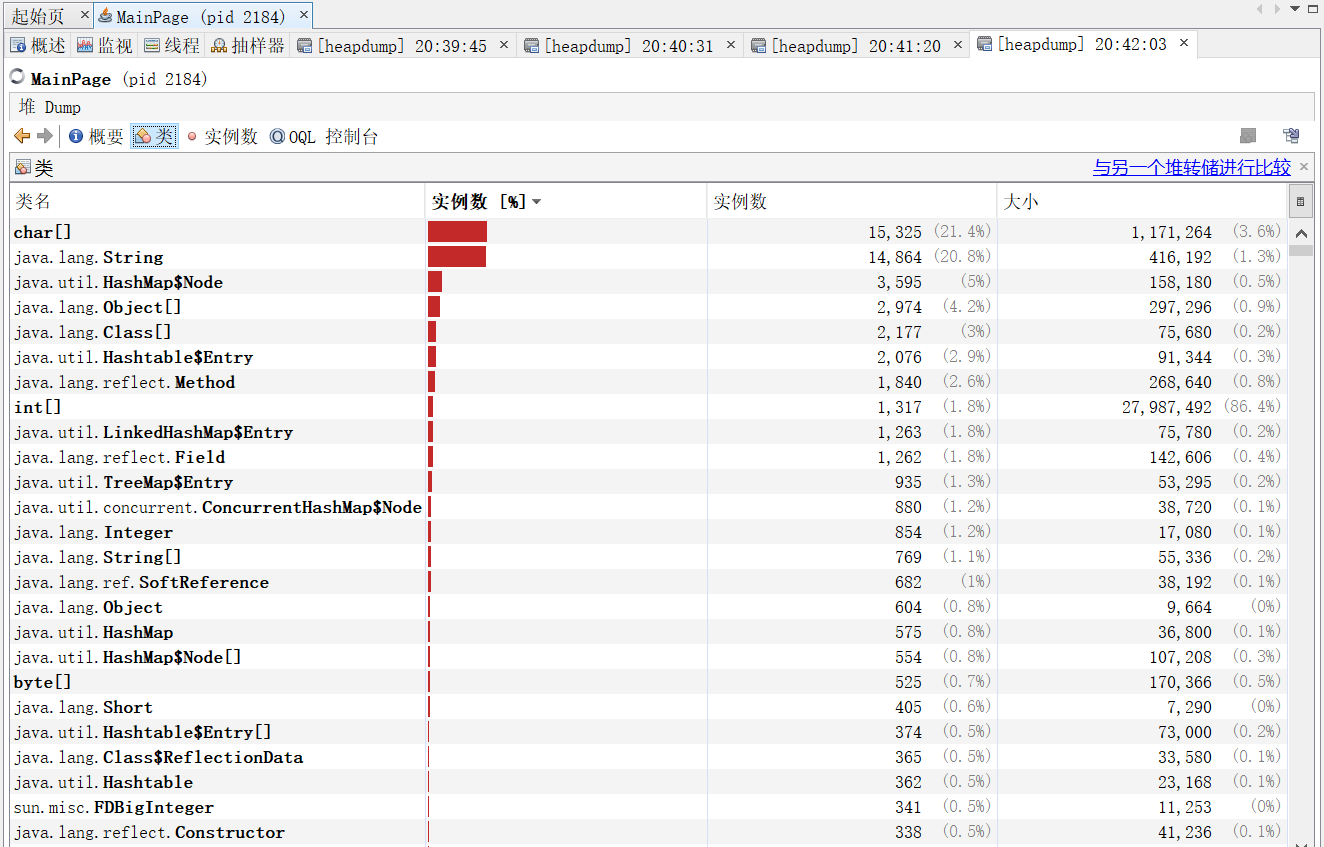
\includegraphics[width=12cm]{/../figures/new-mm-4}
\caption{计算最短路径的堆使用}
\label{fig:new-mm-4}
\end{figure}

\begin{figure}
\centering
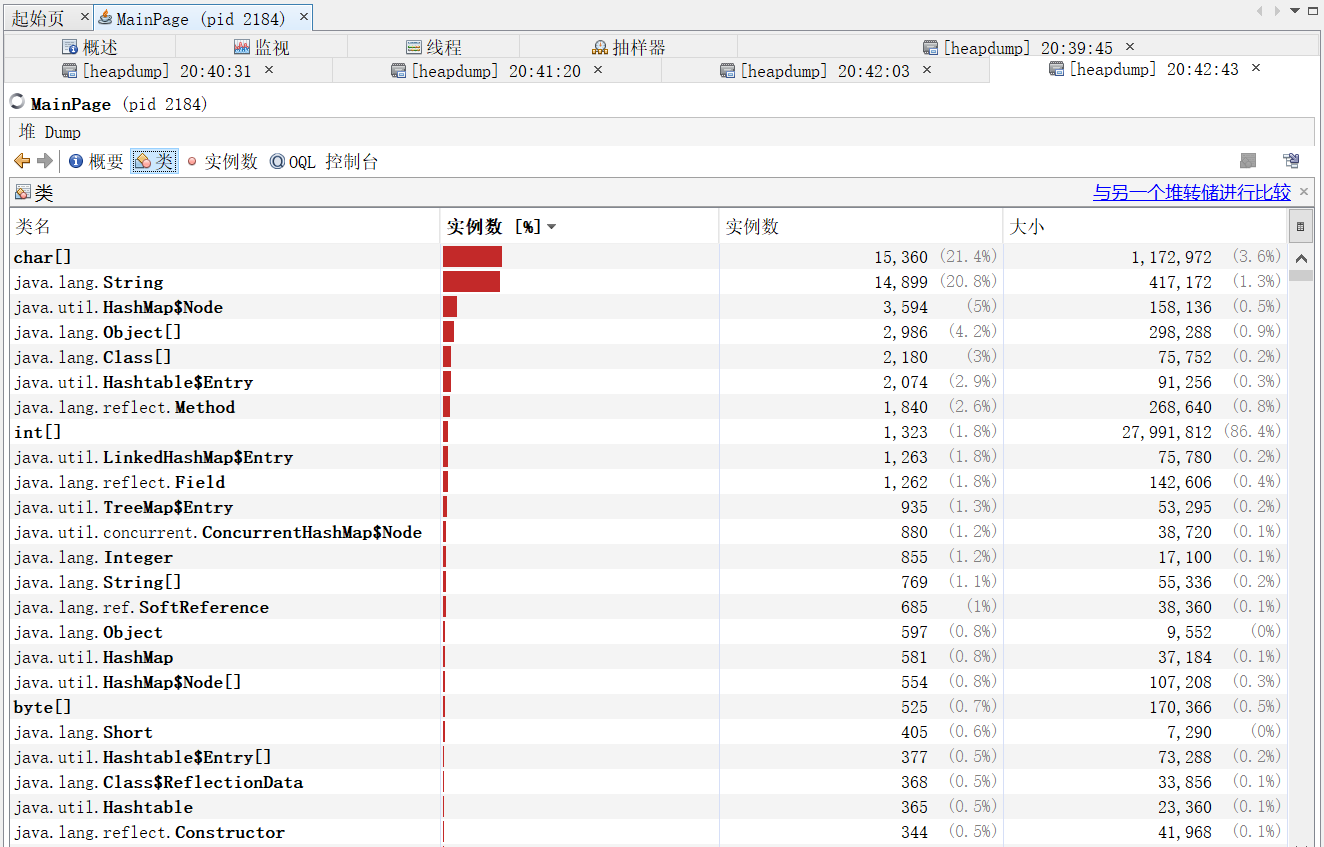
\includegraphics[width=12cm]{/../figures/new-mm-5}
\caption{随机游走的堆使用}
\label{fig:new-mm-5}
\end{figure}

% -------------------------------章节分割线-------------------------------
\BiChapter{利用Git/GitHub进行协作的过程}{}
本章中将描述在本次实验的第一,第二部分中利用Git与GitHub进行协作的截图与相应描述。

\BiSection{第一部分}{}
首先,需要在GitHub上找到待评审代码,fork至本组GitHub仓库内并重命名为Lab4,完成后截图见图\ref{fig:gh-1-1}。

\begin{figure}
\centering
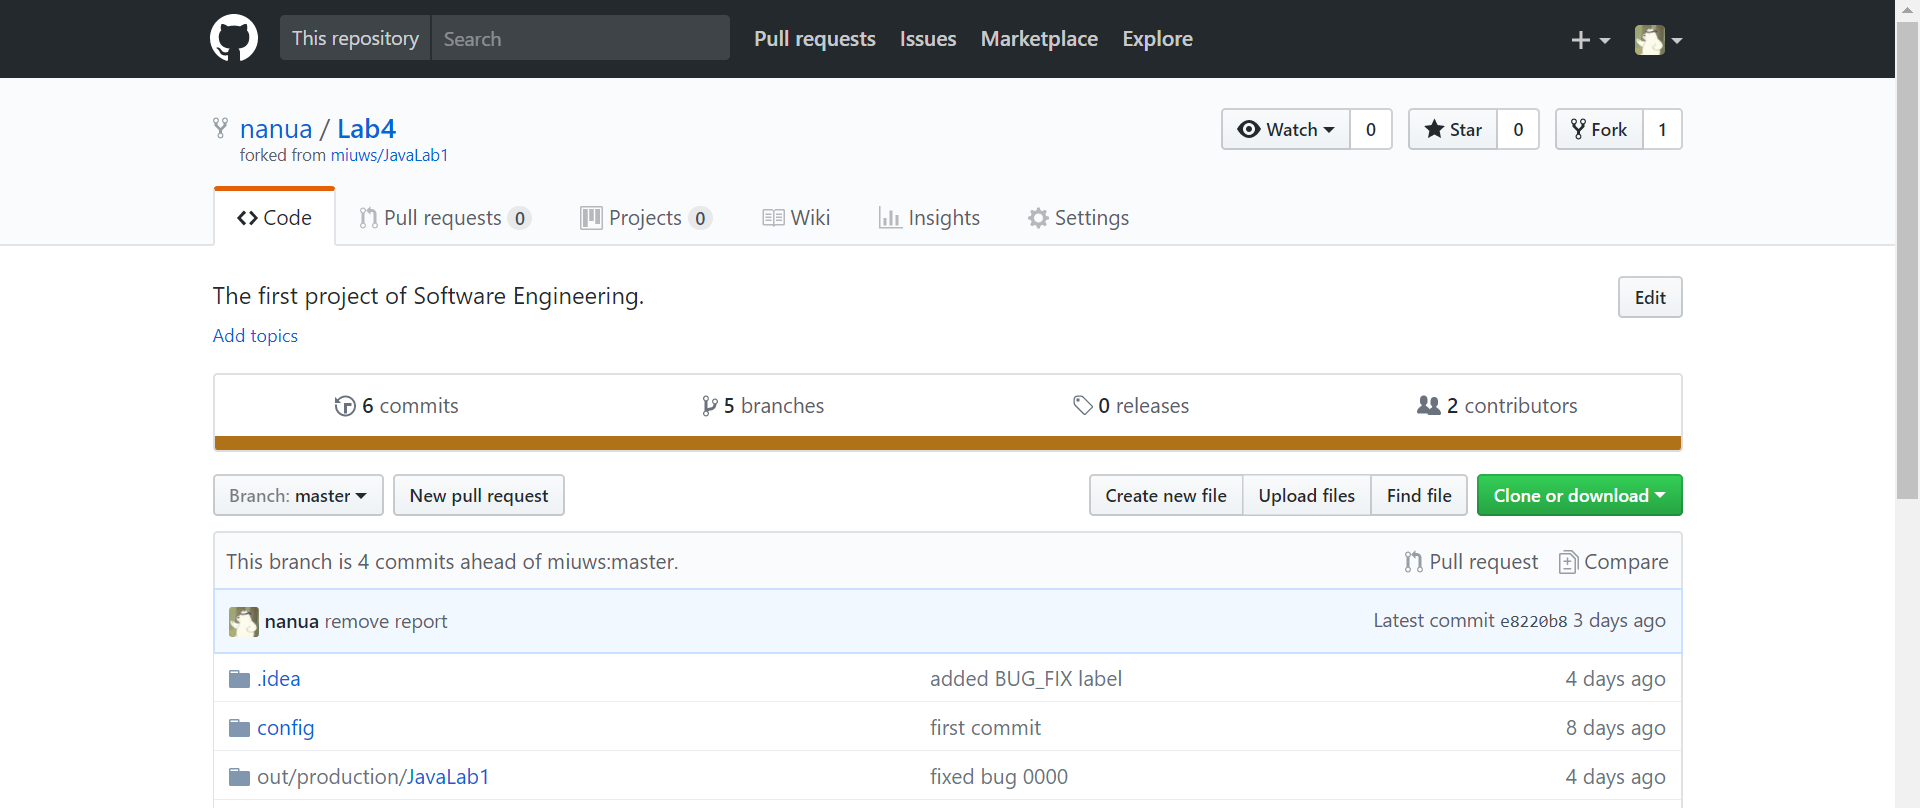
\includegraphics[width=12cm]{/../figures/gh-1-1}
\caption{Fork代评审代码至本组仓库}
\label{fig:gh-1-1}
\end{figure}

然后,将fork得到的仓库Lab4 clone至本组的本地仓库Lab4,完成后截图见图\ref{fig:gh-1-2}。

\begin{figure}
\centering
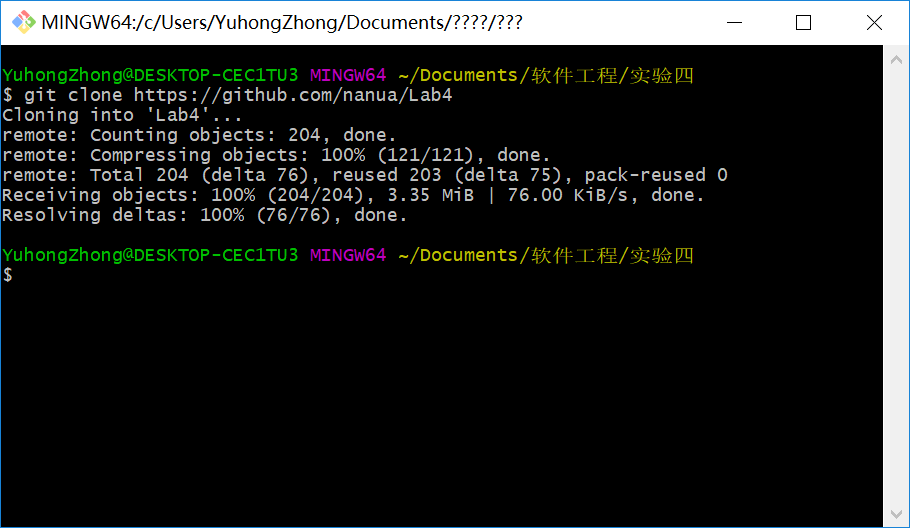
\includegraphics[width=12cm]{/../figures/gh-1-2}
\caption{将远程仓库clone到本地}
\label{fig:gh-1-2}
\end{figure}

完成clone之后,人工review和工具review之后将修改提交至本地仓库,完成后截图见图\ref{fig:gh-1-3}。

\begin{figure}
\centering
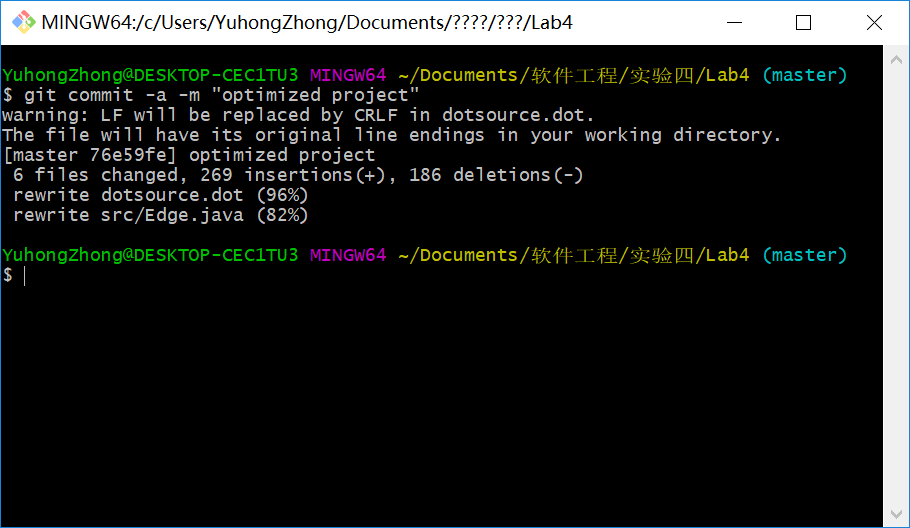
\includegraphics[width=12cm]{/../figures/gh-1-3}
\caption{将修改提交至本地仓库}
\label{fig:gh-1-3}
\end{figure}

提交至本地仓库后,将所有修改历史push到GitHub上本组仓库Lab4,完成后截图见图\ref{fig:gh-1-4}。

\begin{figure}
\centering
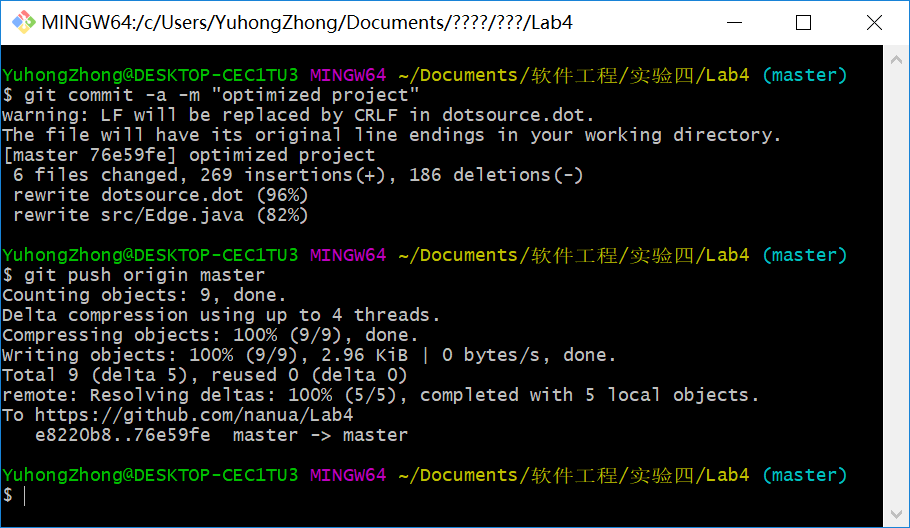
\includegraphics[width=12cm]{/../figures/gh-1-4}
\caption{将本地仓库内容push至远程仓库}
\label{fig:gh-1-4}
\end{figure}

Push至远程仓库后,在Github上将最新的提交Pull Request到原作者的Lab1仓库,完成后截图见图\ref{fig:gh-1-5}。

\begin{figure}
\centering
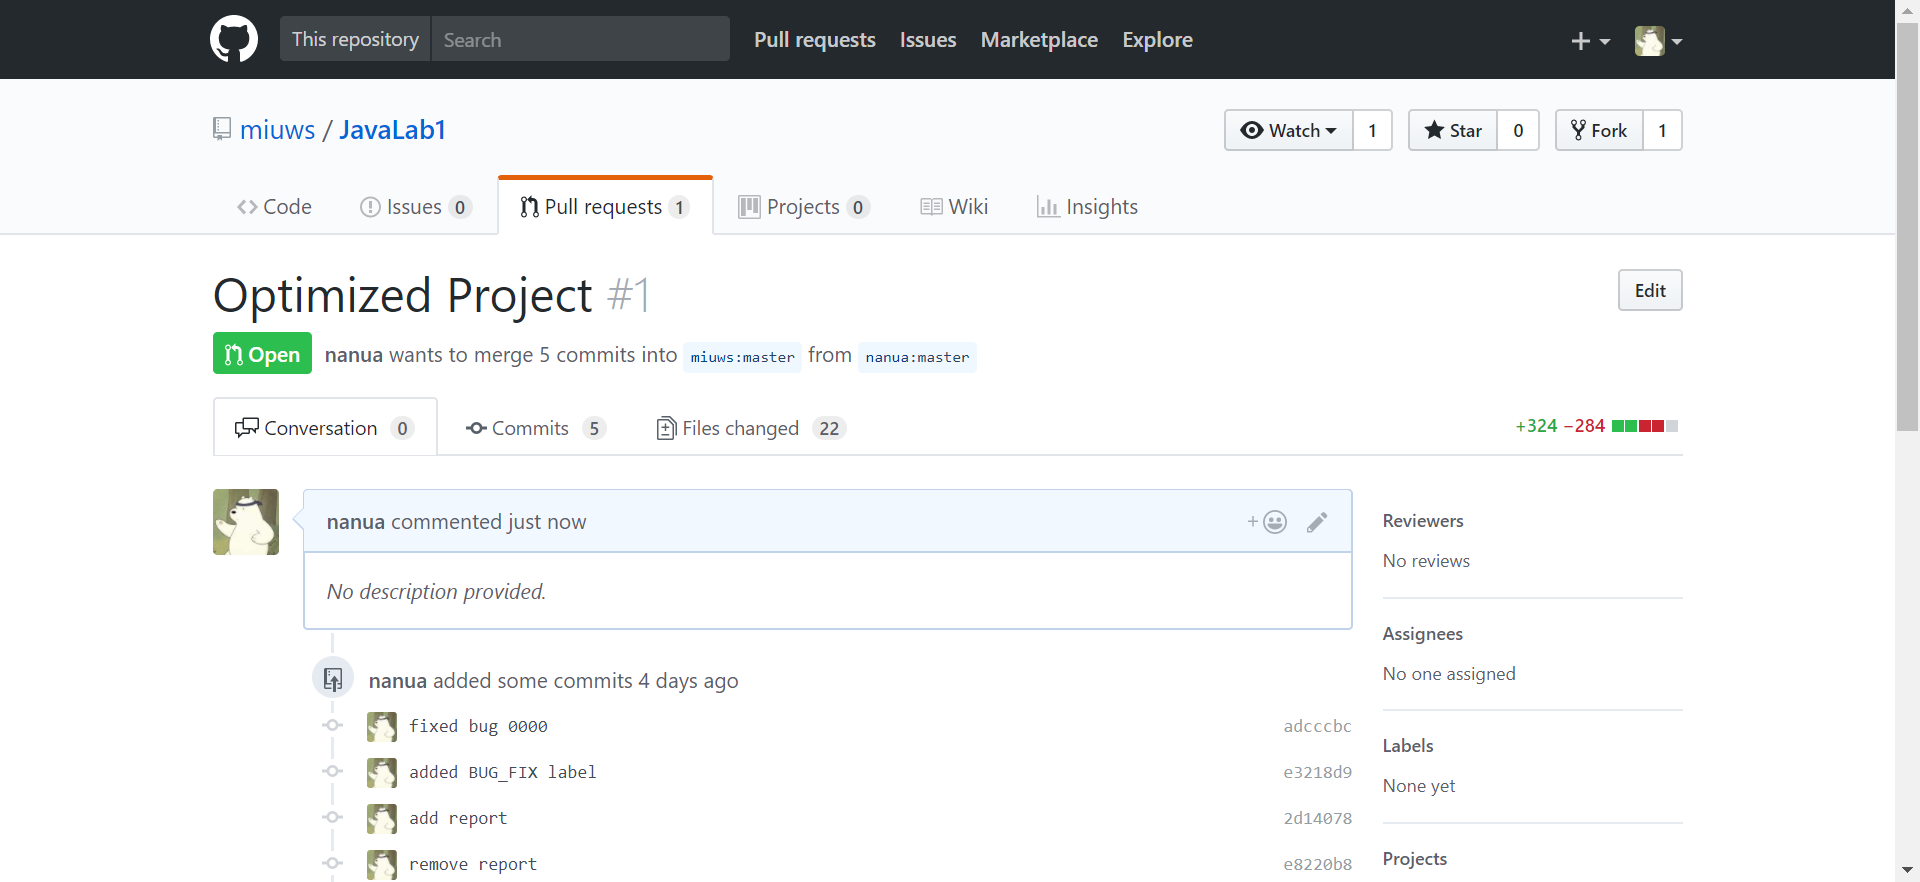
\includegraphics[width=12cm]{/../figures/gh-1-5}
\caption{提交Pull Request}
\label{fig:gh-1-5}
\end{figure}

由此,即完成了利用Git与GitHub进行协作的第一部分。

\BiSection{第二部分}{}
首先,需要原作者在自己的Lab1仓库建立新分支Lab4,建立好后见图\ref{fig:gh-2-1},然后将评审组pull request过来的代码合并进去,合并好后见图\ref{fig:gh-2-2},最后需要将Lab4的分支通过“git fetch”命令fetch到本地Lab1仓库中,fetch完成后见图\ref{fig:gh-2-3}。

\begin{figure}
\centering
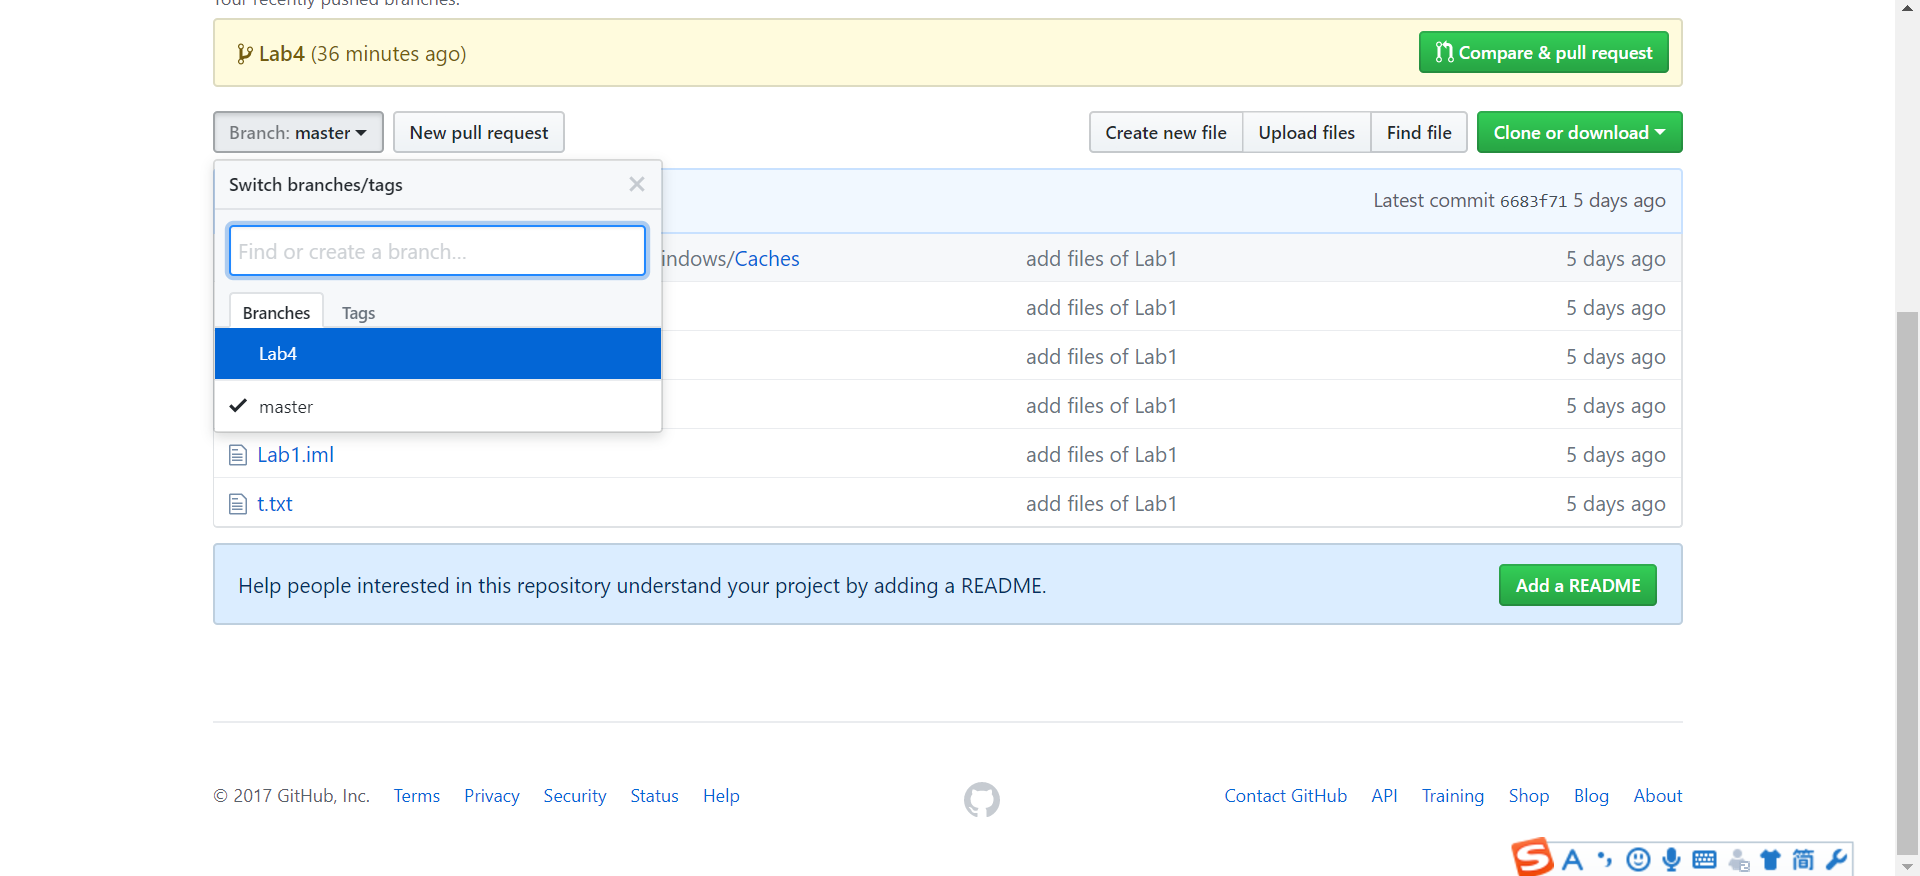
\includegraphics[width=12cm]{/../figures/gh-2-1}
\caption{在远程仓库建立Lab4分支}
\label{fig:gh-2-1}
\end{figure}

\begin{figure}
\centering
\includegraphics[width=12cm]{/../figures/gh-2-2}
\caption{接收评审组的pull request并进行合并}
\label{fig:gh-2-2}
\end{figure}

\begin{figure}
\centering
\includegraphics[width=12cm]{/../figures/gh-2-3}
\caption{将远程Lab4分支fetch到本地}
\label{fig:gh-2-3}
\end{figure}

然后,需要在本地使用git命令“git diff Lab4 master”列出所有的修改,所有修改见图\ref{fig:gh-2-5-1},图\ref{fig:gh-2-5-2},图\ref{fig:gh-2-5-3},图\ref{fig:gh-2-5-4},图\ref{fig:gh-2-5-5},图\ref{fig:gh-2-5-6},图\ref{fig:gh-2-5-7}。之后,需要对每一项修改进行理解以及确认。

\begin{figure}
\centering
\includegraphics[width=12cm]{/../figures/gh-2-5-1}
\caption{查看所有修改(1)}
\label{fig:gh-2-5-1}
\end{figure}

\begin{figure}
\centering
\includegraphics[width=12cm]{/../figures/gh-2-5-2}
\caption{查看所有修改(2)}
\label{fig:gh-2-5-2}
\end{figure}

\begin{figure}
\centering
\includegraphics[width=12cm]{/../figures/gh-2-5-3}
\caption{查看所有修改(3)}
\label{fig:gh-2-5-3}
\end{figure}

\begin{figure}
\centering
\includegraphics[width=12cm]{/../figures/gh-2-5-4}
\caption{查看所有修改(4)}
\label{fig:gh-2-5-4}
\end{figure}

\begin{figure}
\centering
\includegraphics[width=12cm]{/../figures/gh-2-5-5}
\caption{查看所有修改(5)}
\label{fig:gh-2-5-5}
\end{figure}

\begin{figure}
\centering
\includegraphics[width=12cm]{/../figures/gh-2-5-6}
\caption{查看所有修改(6)}
\label{fig:gh-2-5-6}
\end{figure}

\begin{figure}
\centering
\includegraphics[width=12cm]{/../figures/gh-2-5-7}
\caption{查看所有修改(7)}
\label{fig:gh-2-5-7}
\end{figure}

将评审组的改进进行进一步的修改之后,在Lab4分支上进行提交,提交完成后见图\ref{fig:gh-2-6}。

\begin{figure}
\centering
\includegraphics[width=12cm]{/../figures/gh-2-6}
\caption{对评审组的改进进行修改并提交}
\label{fig:gh-2-6}
\end{figure}

最后,需要将Lab4分支与master分支使用git命令“git merge Lab4”进行merge操作,merge完成后见图\ref{fig:gh-2-7}。并在这之后使用“git push”命令将本地的master分支推送到GitHub上远程的Lab1仓库,完成之后见图\ref{fig:gh-2-8}。

\begin{figure}
\centering
\includegraphics[width=12cm]{/../figures/gh-2-7}
\caption{将Lab4分支merge到master分支}
\label{fig:gh-2-7}
\end{figure}

\begin{figure}
\centering
\includegraphics[width=12cm]{/../figures/gh-2-8}
\caption{将master分支推送至GitHub仓库}
\label{fig:gh-2-8}
\end{figure}

由此,即完成了利用Git进行写作的完成过程。

% -------------------------------章节分割线-------------------------------
\BiChapter{评述}{}
在本章中,将分别从代码的规范性以及代码的性能两个角度来对代码进行总体的评述。

\BiSection{对代码规范方面的评述}{}
在代码规范性方面,从Checkstyle的检测结果可以看出,该项目在代码缩进,代码中增加可读性的空格,JavaDoc,大括号的位置,变量名的命名,控制流程的复杂度,Java的语言习惯,限制变量为final,限制方法为final,使用常数变量代替数字,包的导入方式,每行最大字符数等当面皆存在较大的问题,代码风格与Java的标准风格(在测试中采用了Sun以及Google的代码规范)要求差别较大。通过观察可以看出,其代码的规范类似于C语言,并不是Java语言常用的规范,因此可以推断出项目作者对C语言编程较为熟练,但是缺少Java语言的编程训练,将不少C语言中的习惯代入到Java语言的编码过程之中,降低了代码的可读性。特别需要强调的是,除去仅仅影响阅读的缩进,空格等问题之外,该项目中还存在不少的可能影响软件整体的代码缺陷,如在项目中使用数字而不是常值变量,常值变量未声明为final,仅仅在类内部使用的方法未声明为private等。虽然说这些缺陷并不影响代码目前的功能,但是并不利用项目日后的迭代,同时也降低了代码的可维护性,即提高了代码的维护成本。

\BiSection{对代码性能方面的评述}{}
以下将从代码的时间性能,内存性能,以及健壮性三个方面对代码的性能进行评述。

在代码的时间性能方面,从VisualVM的测试结果可以看出,其时间性能主要受到GraphViz绘图程序以及GUI配置函数的限制,其主要的业务逻辑在耗时测试中的占用时间几乎都可以忽略不计,因此若要大幅度的改进项目的时间性能,因考虑采用其他方式进行图片的绘制以及优化GUI的实现方法。在内存性能方面,经过VisualVM的测试,可以推断出在大多数情况下改项目都不会发生内存泄漏的问题,并且占用内存的主要对象也并不是程序中自行创建的对象。并且通过评测数据可以判断其对内存的占用较小,有较好的内存性能。在代码的健壮性方面,有review的结果可知,代码中仍然存在着不够健壮的部分,如点击按钮关闭窗口程序后主线程仍然在运行,在从菜单栏打开功能弹窗后若在弹窗中输入信息再重新打开弹窗则会出现UI元素绘制异常,没有考虑单词中含GraphViz关键字时的处理等问题,因此其健壮性只能满足较低的健壮性要求,并不能很好的处理稍微异常的情况。

% -------------------------------章节分割线-------------------------------
\BiChapter{计划与实际进度}{}
在本节中将描述本次实验中各个环节的任务名称,计划时间长度,实际耗费时间,以及提前或延期的原因分析。
\LTXtable{\textwidth}{body/plan.tex}

% -------------------------------章节分割线-------------------------------
\BiChapter{小结}{}
FindBugs,PMD,CheckStyles三者都是代码规范的静态检查程序,但是在具体的检查要求上它们三者并不相同。就检查的文件而言,PMD和CheckStyles检查的是程序的源文件,而FindBugs检查的则是.class的Java字节码程序。并且,这三者在检查的目的上也并不相同。FindBugs主要检查Java字节码程序中潜在的Bug,如没有合理的关闭资源,使用了错误的相等判断,没有检查空指针等问题。而CheckStyles则是注重检查源代码中的代码规范,如JavaDoc注释,变量的命名规范,import规范,缩进,大括号的位置,有利于阅读的空格等。PMD则是检查代码中的代码规范以及违法最佳实践的情景,如空的catch语句块,过于复杂的控制逻辑,没有发生改变但是没有声明为final的变量等。因此三者虽然都是代码的静态检查程序,但是其检查的文件以及检查的目的皆不一样。在效果方面,由于本次评审的项目代码规范方面有较大的缺陷,因此通过CheckStyles发现了大量的此类问题,并且这其中有部分问题也被PMD所发现。PMD则发现了较多的代码规范以及可能引起问题的代码。而FindBugs则主要发现了资源未释放以及部分编码函数没有指定编码的问题。因此,可以说这三个工具在本次代码评审中皆在不同方面发挥了较大的作用,不过由于本次代码的问题主要集中在代码规范上,因此CheckStyles发挥的作用较大。

在配置以及使用的简易性方面,得益于IntelliJ插件的内部集成,我们都可以在IntelliJ中十分方便的安装以及使用FindBugs,PMD,CheckStyles这三个工具。并且由于所有的工具都有内置的规则集,因此在没有特殊需求时都可以非常简便的直接使用默认的规则集合对待评审的代码进行审查。在代码规范的可扩展性与自定义性方面,PMD,CheckStyles都可以非常简易的导入自行编写的规则集,但是FindBugs则需要从FindBugs的源码入手进行修改,添加自定义的规则,然后将编译好的jar文件替代原来的FindBugs程序。因此从可扩展性的角度讲,PMD与CheckStyles要优于FindBugs。

在本次实验中,主要使用VisualVM进行代码的时间性能评测以及空间性能评测。VisualVM都以图表的方式直观的显示出了测试时间段内程序中各个函数的运行耗时以及各个类的实例所占用的堆空间。特别值得一提的时,VisualVM的计时是针对函数执行的时间进行记录的,并不是程序的执行时间,因此能够给我们更加细致的程序时间性能的分析,而且VisualVM能够支持随时通过按钮进行垃圾回收,由此避免了在不同时间点测试堆的占用图像时由于未回收的垃圾对分析造成的影响。在结果方面,VisualVM发现了本次评审的代码中耗费时间的主要是GUI元素的配置以及调用GraphViz进行绘图的操作,给如何提升程序的时间性能提供了足够的信息。并且,在空间性能方面,也通过VisualVM的分析报告推断出项目中基本不存在内存泄漏问题,因此不需要对内存泄漏进行进一步的改进,减少了代码优化时需要考虑的问题。

对于代码是否符合规范与代码执行的时空复杂性方面,我们认为两者之间并不存在必然的直接联系。因为代码规范是编写代码的一种最佳实践,即符合此规范的代码更有可能具备较好的性能(也即包括了时空复杂性),但是并不是说代码符合规范就一定有较好的时空复杂性,或代码有较好的时空复杂性就一定很好的符合了规范,后者的典型反例即为各类编程竞赛中选手的代码。并且,代码规范能够使得软件更有可能有较好的性能,其中的性能并不只是时空复杂性,还包括了健壮性,可维护性,可读性等工程方面的问题。不过,具备较好时空复杂性的代码一般都较好地符合了代码规范,因为否则可能造成内存泄漏等问题,从而严重影响代码的时空性能。综上所述,我们认为虽然这两者之间没有必然的直接联系,但是两者之间仍然相互依赖。

在软件代码优化方面,通过这次的实验,我们认识到代码的评审与优化既不能离开人工审核,也不能放弃使用代码自动评审工具。自动评审工具能够执行大量繁琐机器规则检查,避免人工进行这些规则检查时由于疏忽而忽略的问题,而人工评审则能够编写多种多样的测试用例去测试各种极端情况以及各种组合情况,由此共同配合去发现代码中已经出现的错误及极有可能出现错误的位置,进而优化代码的性能。

%%% Local Variables:
%%% mode: latex
%%% TeX-master: "../main"
%%% End:
